\documentclass[uplatex,a4j,11pt,dvipdfmx]{jsarticle}
\bibliographystyle{jplain}

\usepackage{url}

\usepackage{graphicx}
\usepackage{gnuplot-lua-tikz}
\usepackage{pgfplots}
\usepackage{tikz}
\usepackage{amsmath,amsfonts,amssymb}
\usepackage{bm}
\usepackage{siunitx}

\makeatletter
\def\fgcaption{\def\@captype{figure}\caption}
\makeatother
\newcommand{\setsections}[3]{
\setcounter{section}{#1}
\setcounter{subsection}{#2}
\setcounter{subsubsection}{#3}
}
\newcommand{\mfig}[3][width=15cm]{
\begin{center}
\includegraphics[#1]{#2}
\fgcaption{#3 \label{fig:#2}}
\end{center}
}

\begin{document}
%\begin{tikzpicture}[gnuplot]
%% generated with GNUPLOT 5.2p8 (Lua 5.3; terminal rev. Nov 2018, script rev. 108)
%% 2021年07月30日 15時10分02秒
\path (0.000,0.000) rectangle (10.000,8.000);
\gpcolor{color=gp lt color border}
\gpsetlinetype{gp lt border}
\gpsetdashtype{gp dt solid}
\gpsetlinewidth{1.00}
\draw[gp path] (2.030,0.985)--(2.210,0.985);
\draw[gp path] (8.737,0.985)--(8.557,0.985);
\node[gp node right] at (1.846,0.985) {$-20$};
\draw[gp path] (2.030,2.103)--(2.210,2.103);
\draw[gp path] (8.737,2.103)--(8.557,2.103);
\node[gp node right] at (1.846,2.103) {$-10$};
\draw[gp path] (2.030,3.220)--(2.210,3.220);
\draw[gp path] (8.737,3.220)--(8.557,3.220);
\node[gp node right] at (1.846,3.220) {$0$};
\draw[gp path] (2.030,4.338)--(2.210,4.338);
\draw[gp path] (8.737,4.338)--(8.557,4.338);
\node[gp node right] at (1.846,4.338) {$10$};
\draw[gp path] (2.030,5.456)--(2.210,5.456);
\draw[gp path] (8.737,5.456)--(8.557,5.456);
\node[gp node right] at (1.846,5.456) {$20$};
\draw[gp path] (2.030,6.573)--(2.210,6.573);
\draw[gp path] (8.737,6.573)--(8.557,6.573);
\node[gp node right] at (1.846,6.573) {$30$};
\draw[gp path] (2.030,7.691)--(2.210,7.691);
\draw[gp path] (8.737,7.691)--(8.557,7.691);
\node[gp node right] at (1.846,7.691) {$40$};
\draw[gp path] (2.030,0.985)--(2.030,1.165);
\draw[gp path] (2.030,7.691)--(2.030,7.511);
\node[gp node center] at (2.030,0.677) {$-4$};
\draw[gp path] (3.371,0.985)--(3.371,1.165);
\draw[gp path] (3.371,7.691)--(3.371,7.511);
\node[gp node center] at (3.371,0.677) {$-2$};
\draw[gp path] (4.713,0.985)--(4.713,1.165);
\draw[gp path] (4.713,7.691)--(4.713,7.511);
\node[gp node center] at (4.713,0.677) {$0$};
\draw[gp path] (6.054,0.985)--(6.054,1.165);
\draw[gp path] (6.054,7.691)--(6.054,7.511);
\node[gp node center] at (6.054,0.677) {$2$};
\draw[gp path] (7.396,0.985)--(7.396,1.165);
\draw[gp path] (7.396,7.691)--(7.396,7.511);
\node[gp node center] at (7.396,0.677) {$4$};
\draw[gp path] (8.737,0.985)--(8.737,1.165);
\draw[gp path] (8.737,7.691)--(8.737,7.511);
\node[gp node center] at (8.737,0.677) {$6$};
\draw[gp path] (2.030,7.691)--(2.030,0.985)--(8.737,0.985)--(8.737,7.691)--cycle;
\node[gp node center,rotate=-270] at (1.002,4.338) {$y$};
\node[gp node center] at (5.383,0.215) {$x$};
\gpcolor{rgb color={0.580,0.000,0.827}}
\gpsetpointsize{4.00}
\gppoint{gp mark 1}{(2.030,2.143)}
\gppoint{gp mark 1}{(2.097,2.084)}
\gppoint{gp mark 1}{(2.164,2.260)}
\gppoint{gp mark 1}{(2.231,2.106)}
\gppoint{gp mark 1}{(2.298,2.267)}
\gppoint{gp mark 1}{(2.365,2.284)}
\gppoint{gp mark 1}{(2.432,2.425)}
\gppoint{gp mark 1}{(2.499,2.476)}
\gppoint{gp mark 1}{(2.567,2.446)}
\gppoint{gp mark 1}{(2.634,2.468)}
\gppoint{gp mark 1}{(2.701,2.982)}
\gppoint{gp mark 1}{(2.768,2.507)}
\gppoint{gp mark 1}{(2.835,2.899)}
\gppoint{gp mark 1}{(2.902,2.972)}
\gppoint{gp mark 1}{(2.969,2.890)}
\gppoint{gp mark 1}{(3.036,2.831)}
\gppoint{gp mark 1}{(3.103,3.103)}
\gppoint{gp mark 1}{(3.170,3.037)}
\gppoint{gp mark 1}{(3.237,3.086)}
\gppoint{gp mark 1}{(3.304,2.991)}
\gppoint{gp mark 1}{(3.371,3.095)}
\gppoint{gp mark 1}{(3.438,3.181)}
\gppoint{gp mark 1}{(3.506,3.474)}
\gppoint{gp mark 1}{(3.573,3.352)}
\gppoint{gp mark 1}{(3.640,3.363)}
\gppoint{gp mark 1}{(3.707,3.565)}
\gppoint{gp mark 1}{(3.774,3.382)}
\gppoint{gp mark 1}{(3.841,3.655)}
\gppoint{gp mark 1}{(3.908,3.700)}
\gppoint{gp mark 1}{(3.975,3.777)}
\gppoint{gp mark 1}{(4.042,3.744)}
\gppoint{gp mark 1}{(4.109,3.794)}
\gppoint{gp mark 1}{(4.176,3.846)}
\gppoint{gp mark 1}{(4.243,3.791)}
\gppoint{gp mark 1}{(4.310,3.890)}
\gppoint{gp mark 1}{(4.377,4.089)}
\gppoint{gp mark 1}{(4.445,4.055)}
\gppoint{gp mark 1}{(4.512,4.129)}
\gppoint{gp mark 1}{(4.579,4.049)}
\gppoint{gp mark 1}{(4.646,4.366)}
\gppoint{gp mark 1}{(4.713,4.422)}
\gppoint{gp mark 1}{(4.780,4.296)}
\gppoint{gp mark 1}{(4.847,4.510)}
\gppoint{gp mark 1}{(4.914,4.386)}
\gppoint{gp mark 1}{(4.981,4.412)}
\gppoint{gp mark 1}{(5.048,4.600)}
\gppoint{gp mark 1}{(5.115,4.594)}
\gppoint{gp mark 1}{(5.182,4.663)}
\gppoint{gp mark 1}{(5.249,4.646)}
\gppoint{gp mark 1}{(5.316,4.789)}
\gppoint{gp mark 1}{(5.384,5.029)}
\gppoint{gp mark 1}{(5.451,4.936)}
\gppoint{gp mark 1}{(5.518,4.860)}
\gppoint{gp mark 1}{(5.585,5.108)}
\gppoint{gp mark 1}{(5.652,5.228)}
\gppoint{gp mark 1}{(5.719,5.249)}
\gppoint{gp mark 1}{(5.786,5.372)}
\gppoint{gp mark 1}{(5.853,5.490)}
\gppoint{gp mark 1}{(5.920,5.405)}
\gppoint{gp mark 1}{(5.987,5.283)}
\gppoint{gp mark 1}{(6.054,5.625)}
\gppoint{gp mark 1}{(6.121,5.379)}
\gppoint{gp mark 1}{(6.188,5.560)}
\gppoint{gp mark 1}{(6.255,5.689)}
\gppoint{gp mark 1}{(6.322,5.742)}
\gppoint{gp mark 1}{(6.390,5.909)}
\gppoint{gp mark 1}{(6.457,5.907)}
\gppoint{gp mark 1}{(6.524,5.631)}
\gppoint{gp mark 1}{(6.591,5.683)}
\gppoint{gp mark 1}{(6.658,5.746)}
\gppoint{gp mark 1}{(6.725,5.936)}
\gppoint{gp mark 1}{(6.792,6.034)}
\gppoint{gp mark 1}{(6.859,6.334)}
\gppoint{gp mark 1}{(6.926,6.107)}
\gppoint{gp mark 1}{(6.993,6.217)}
\gppoint{gp mark 1}{(7.060,6.188)}
\gppoint{gp mark 1}{(7.127,6.532)}
\gppoint{gp mark 1}{(7.194,6.466)}
\gppoint{gp mark 1}{(7.261,6.709)}
\gppoint{gp mark 1}{(7.329,6.392)}
\gppoint{gp mark 1}{(7.396,6.456)}
\gppoint{gp mark 1}{(7.463,6.857)}
\gppoint{gp mark 1}{(7.530,6.685)}
\gppoint{gp mark 1}{(7.597,6.779)}
\gppoint{gp mark 1}{(7.664,6.799)}
\gppoint{gp mark 1}{(7.731,6.879)}
\gppoint{gp mark 1}{(7.798,6.737)}
\gppoint{gp mark 1}{(7.865,7.068)}
\gppoint{gp mark 1}{(7.932,7.154)}
\gppoint{gp mark 1}{(7.999,7.033)}
\gppoint{gp mark 1}{(8.066,7.080)}
\gppoint{gp mark 1}{(8.133,7.222)}
\gppoint{gp mark 1}{(8.200,7.301)}
\gppoint{gp mark 1}{(8.268,7.174)}
\gppoint{gp mark 1}{(8.335,7.347)}
\gppoint{gp mark 1}{(8.402,7.330)}
\gppoint{gp mark 1}{(8.469,7.406)}
\gppoint{gp mark 1}{(8.536,7.234)}
\gppoint{gp mark 1}{(8.603,7.549)}
\gppoint{gp mark 1}{(8.670,7.584)}
\gppoint{gp mark 1}{(8.737,7.668)}
\gpcolor{rgb color={0.000,0.620,0.451}}
\draw[gp path] (2.030,2.080)--(2.098,2.137)--(2.165,2.193)--(2.233,2.250)--(2.301,2.306)%
  --(2.369,2.363)--(2.436,2.419)--(2.504,2.475)--(2.572,2.532)--(2.640,2.588)--(2.707,2.645)%
  --(2.775,2.701)--(2.843,2.758)--(2.911,2.814)--(2.978,2.871)--(3.046,2.927)--(3.114,2.983)%
  --(3.182,3.040)--(3.249,3.096)--(3.317,3.153)--(3.385,3.209)--(3.453,3.266)--(3.520,3.322)%
  --(3.588,3.379)--(3.656,3.435)--(3.724,3.492)--(3.791,3.548)--(3.859,3.604)--(3.927,3.661)%
  --(3.995,3.717)--(4.062,3.774)--(4.130,3.830)--(4.198,3.887)--(4.266,3.943)--(4.333,4.000)%
  --(4.401,4.056)--(4.469,4.112)--(4.537,4.169)--(4.604,4.225)--(4.672,4.282)--(4.740,4.338)%
  --(4.808,4.395)--(4.875,4.451)--(4.943,4.508)--(5.011,4.564)--(5.079,4.620)--(5.146,4.677)%
  --(5.214,4.733)--(5.282,4.790)--(5.350,4.846)--(5.417,4.903)--(5.485,4.959)--(5.553,5.016)%
  --(5.621,5.072)--(5.688,5.128)--(5.756,5.185)--(5.824,5.241)--(5.892,5.298)--(5.959,5.354)%
  --(6.027,5.411)--(6.095,5.467)--(6.163,5.524)--(6.230,5.580)--(6.298,5.637)--(6.366,5.693)%
  --(6.434,5.749)--(6.501,5.806)--(6.569,5.862)--(6.637,5.919)--(6.705,5.975)--(6.772,6.032)%
  --(6.840,6.088)--(6.908,6.145)--(6.976,6.201)--(7.043,6.257)--(7.111,6.314)--(7.179,6.370)%
  --(7.247,6.427)--(7.314,6.483)--(7.382,6.540)--(7.450,6.596)--(7.518,6.653)--(7.585,6.709)%
  --(7.653,6.765)--(7.721,6.822)--(7.789,6.878)--(7.856,6.935)--(7.924,6.991)--(7.992,7.048)%
  --(8.060,7.104)--(8.127,7.161)--(8.195,7.217)--(8.263,7.274)--(8.331,7.330)--(8.398,7.386)%
  --(8.466,7.443)--(8.534,7.499)--(8.602,7.556)--(8.669,7.612)--(8.737,7.669);
\gpcolor{color=gp lt color border}
\draw[gp path] (2.030,7.691)--(2.030,0.985)--(8.737,0.985)--(8.737,7.691)--cycle;
%% coordinates of the plot area
\gpdefrectangularnode{gp plot 1}{\pgfpoint{2.030cm}{0.985cm}}{\pgfpoint{8.737cm}{7.691cm}}
\end{tikzpicture}
%% gnuplot variables

%\section{実験装置, 試料について}
\subsection{分光計について}
分光計の模式図を図\ref{fig:fig/fig2.png}に示す.
有限の幅を持ったスリット$S_1$から入射した光が回折格子で反射し$S_2$から出る.
このとき入射角$\alpha=\gamma+\theta$, 出射角$\beta=\gamma-\theta$であり,それぞれ$\delta\alpha$, $\delta\beta$の幅を持つ.
ここで回折条件は格子定数$d$として
\begin{align}
  \begin{split}
    \lambda\pm\delta\lambda&=d|\sin(\alpha\pm\delta\alpha)-\sin(\beta\pm\delta\beta)|\\
    &\simeq d|\sin\alpha-\sin\beta\pm(\cos\alpha\delta\alpha-\cos\beta\delta\beta)|\\
  \end{split}
\end{align}
となる.ここで$\delta\alpha,\delta\beta\ll1$として近似した.
$\lambda$に関する部分を見ると
\begin{align}
  \begin{split}
    \pm\lambda&=d(\sin\alpha-\sin\beta)\\
    &=2d\sin\theta\cos\gamma
  \end{split}
\end{align}
となり,回折格子を回転させることで任意の波長の光を取り出せることがわかる.
また$\delta\lambda$に関する部分を見ると
\begin{align}
    \delta\lambda&=d|\cos\alpha\delta\alpha-\cos\beta\delta\beta|
\end{align}
ここで誤差の伝搬則を用いると
\begin{align}
  |\delta\lambda|=d\sqrt{(\cos\alpha\delta\alpha)^2+(\cos\beta\delta\beta)^2}
\end{align}
となる.ここで幾何学的に
\begin{align}
  F\delta\alpha\simeq x_1\cos\gamma
\end{align}
なので$x_1=x_2=x$のもとで
\begin{align}
  |\delta\lambda|=d\sqrt{\left(\frac{x\cos\gamma}{F}\cos\alpha\right)^2+\left(\frac{x\cos\gamma}{F}\cos\beta\right)^2}
\end{align}
さらに$\gamma,\alpha,\beta\ll1$と仮定するとスペクトルの幅は以下のようになる.
\begin{align}
  |\delta\lambda|\simeq \frac{\sqrt{2}d}{F}x
\end{align}

分光計に単色光を入射した場合の出力が半値幅$2|\delta\lambda|$すなわち$\sigma_a=\delta\lambda/2\sqrt{2\ln 2}$のガウス関数であるとする.
このとき$\sigma_\lambda$のガウス関数型スペクトルを持った光を入射すると,その出力のスペクトル$H$は以下の畳み込み積分で表される.
\begin{align}
  \begin{split}
    H(\lambda)&=\int_{-\infty}^{\infty}\frac{1}{2\pi\sigma_a\sigma_\lambda}{\rm e}^{-(t/\sqrt{2}\sigma_a)^2}{\rm e}^{-((\lambda-t)/\sqrt{2}\sigma_\lambda)^2}{\rm d}t\\
    &=\frac{{\rm e}^{-\lambda^2/2(\sigma_a^2+\sigma_\lambda^2)}}{2\pi\sigma_a\sigma_\lambda}\int^\infty_{-\infty}\exp\left(-\frac{\sigma_a^2+\sigma_\lambda^2}{2\sigma_a^2\sigma_\lambda^2}\left(t-\frac{\sigma_a^2\sigma_\lambda^2}{\sigma_a^2+\sigma_\lambda^2}\frac{\lambda}{\sigma_\lambda^2}\right)^2\right)\\
    &=\frac{1}{\sqrt{2\pi(\sigma_a^2+\sigma_\lambda^2)}}\exp\left(-\frac{t^2}{2(\sigma_a^2+\sigma_\lambda^2)}\right)
  \end{split}
\end{align}
すなわちガウス関数型のスペクトル分布を持った光を分光器に入力した場合も同様にガウス関数型のスペクトルが得られることがわかる.
\mfig[width=6cm]{fig/fig2.png}{分光計の模式図}
\subsection{FPIについて}
Fabry-Perrot Interderometer (FPI, ファブリ・ペロー干渉計)は任意の波長を選択的に取り出す光学機器である.
図\ref{fig:fig/fig3.png}にFPIの模式図を示す.
2つの半透鏡が向かいあわせに設置され,共振器長$D$が可変できるようになっている.
このとき周波数$\nu$の光が共振器内で定在波として存在する条件は
\begin{align}
  \nu_m=\frac{mc}{2D}\qquad(m\in\mathbb{N})
\end{align}
であり$D$を可変することで特定の波長を選択的に取り出すことができる.
$D$を一定の速度で掃引するとモードの異なるスペクトルパターンが周期的に現れ,これを測定することでスペクトルを高い分解能で測定できる.

FPIを用いてHe-Neレーザーのスペクトルを調べることを考える.
He-Neレーザーは多モード発振しておりそのここでは$\lambda_1$と$\lambda_2$にピークを持つとする.
したがってFPIスペクトルは図\ref{fig:He-Ne_FPI}のようになる.したがって以下が成り立つ.
\begin{align}
  \Delta D_1&=\frac{(m+1)\lambda_1}{2}-\frac{m\lambda_1}{2}=\frac{\lambda_1}{2}\\
  \Delta D_2&=\frac{m\lambda_2}{2}-\frac{m\lambda_1}{2}=\frac{m\Delta\lambda}{2}
\end{align}
ここで実際に測定されるのはピーク間の時間間隔であるが$D$の掃引速度が一定($=v$)であるならば
図\ref{fig:He-Ne_FPI}のように$\Delta_1=vT,\Delta_2=vt$となるので
\begin{align}
  \frac{t}{T}=\frac{\Delta D_2}{\Delta D_1}=\frac{m\Delta\lambda}{\lambda}
\end{align}
である.更に干渉条件$D\sim\frac{m\lambda}{2}$より$m$を消去すると
\begin{align}
  \frac{t}{T}=\frac{2\Delta\lambda}{\lambda^2}D
\end{align}
となるので$\lambda,D$が既知ならば$t/T$から$\Delta\lambda$が求まる.
\begin{figure}[htbp]
  \begin{center}
    \begin{tikzpicture}
      \begin{axis}[ticks=none,
        axis lines=center,
        ymin=0,
        ymax=0.5,
        xmin=1,
        xmax=7,
        ylabel=輻射強度$I$,
        xlabel=共振器長$D$,
        axis line style = thick,
        width=12cm,
        height=7cm,
        ylabel near ticks,
        xlabel near ticks,
        ]
        \draw [] (axis cs:4,0.37) node [above] {$\Delta D_1=vT$};
        \draw [] (axis cs:2.75,0.22) node [above] {$\Delta D_2=vt$};
        \draw [] (axis cs:5.4,0.4) node [above] {$\tfrac{(m+1)\lambda_1}{2}$};
        \draw [] (axis cs:6.1,0.4) node [above] {$\tfrac{(m+1)\lambda_2}{2}$};
        \draw [] (axis cs:2.5,0.4) node [above] {$\tfrac{m\lambda_1}{2}$};
        \draw [] (axis cs:3.0,0.4) node [above] {$\tfrac{m\lambda_2}{2}$};
        \draw[-latex,red] (axis cs:2.5,0) -- (axis cs:2.5,0.35);
        \draw[-latex,red] (axis cs:3,0) -- (axis cs:3,0.2);
        \draw[-latex,red] (axis cs:5.5,0) -- (axis cs:5.5,0.35);
        \draw[-latex,red] (axis cs:6,0) -- (axis cs:6,0.2);
        \draw[latex-latex,black] (axis cs:2.5,0.37) -- (axis cs:5.5,0.37);
        \draw[latex-latex,black] (axis cs:2.5,0.22) -- (axis cs:3,0.22);
      \end{axis}
    \end{tikzpicture}
  \end{center}
  \caption{He-NeレーザーのFPIスペクトル}
  \label{fig:He-Ne_FPI}
\end{figure}
\mfig[width=10cm]{fig/fig3.png}{FPI装置の模式図}
%\subsection*{カーテンウォール(CW)について}
カーテンウォールは高層ビルの発展に伴って19世紀以降に現れた非耐力壁の一種である.
19世紀に鉄骨造が発展し,壁が構造を支える必要性が無くなった.
また高層ビルの建設にあたり,壁の軽量化と高所での作業量を削減する必要があった.
カーテンウォールは非耐力壁であることから,壁の肉厚を削減でき壁の軽量化に寄与する.
更にプレファブ化によって現地での作業量を減らし,また工期短縮や足場の削減に寄与している.
加えてカーテンウォールは生産数が非常に多いことから,カーテンウォールを専門とする製造者が成立するため,
低コスト化や品質の安定化,技術の蓄積が行われやすいなどのメリットがある.
また一棟の高層ビルでも多くのカーテンウォールを使うことから,大規模なビルではオーダーメイドのカーテンウォールを用いて個性を表現することが多い.

カーテンウォールは主に金属系カーテンウォールとPC(プレキャストコンクリート)カーテンウォールに大別される.
金属系のカーテンウォールについてインターネットで検索したところフジテレビ本社ビルが金属系カーテンウォールを用いているとわかった.\cite{2008020675:online}
図\ref{fig:fig/huji.jpg}のように金属系カーテンウォールは金属光沢感が強いことがわかる.
一方でPCカーテンウォールは金属系に比べて重く,新しい技術である.
PCカーテンウォールは図\ref{fig:fig/pc_cw.jpg}のように重厚感のある表現が可能で,またコンクリートが主成分であることから耐火性が高く,重いことから遮音性も高い.
\mfig[width=8cm]{fig/huji.jpg}{フジテレビ本社ビル\cite{LIXIL70:online}}
\mfig[width=8cm]{fig/pc_cw.jpg}{PCカーテンウォール\cite{PC39:online}}

またカーテンウォールはその構造によっても分類でき,主に方立方式とパネル方式に分類される.
方立方式は方立(マリオン)という鉛直向きの枠材を一定ピッチで配置し,その間にガラスやパネルをはめ込むことで構成されるカーテンウォールで,金属系カーテンウォールで主に用いられる.
マリオン方式ではパネルが受ける風圧力などの水平力はマリオンを介して建物に伝達される.
方立方式の建物を検索したところ有楽町マリオンというものがあるとわかった.\cite{yuurakutyo59:online}図\ref{fig:fig/yuurakutyo.jpg}に有楽町マリオンの画像を示す.
画像からも明らかなように有楽町マリオンは方立を前面に押し出したデザインであることがわかる.
またマリオン方式では細長い部材が連続することから,熱による膨張を考慮するべきである.
そこで方立と建物の接続には図のようなファスナーという部品が用いられ,長孔によって変位を吸収するようになっている.
\mfig[width=8cm]{fig/yuurakutyo.jpg}{有楽町マリオン\cite{yuurakutyo59:online}}
\mfig[width=10cm]{fig/marion_fasnar.jpg}{ファスナーの例\cite{SR26:online}}

一方でパネル方式のカーテンウォールは1階分の高さのパネルを方下左右に並べることで構成され,図\ref{fig:fig/huji.jpg}のフジテレビ本社ビルもパネル方式である.\cite{LIXIL70:online}
パネル方式は金属系でもPCでも用いられる方式である.
高層ビルにおいては地震などにより水平力が加わると層の間に水平方向の変位が発生することがあり,これを層間変位と呼ぶ.
方立方式の場合パネルはマリオンを介して接続され,そのマリオンもファスナーによって接続されることから層間変位を吸収するのは比較的容易である.
一方でパネル方式の場合は面内方向の合成が高いパネルが直接建物に接続されることから,層間変位の吸収に特別の考慮が必要である.
層間変位の吸収にはロッキング方式やスライド方式などの方式がある.図\ref{fig:fig/soukan.jpg}に各方式の概略図を示す.
ロッキング方式は図\ref{fig:fig/soukan.jpg}の左側のように各パネルがピンを軸に回転することで層間変位を吸収する.
一方スライド方式は図\ref{fig:fig/soukan.jpg}右側のように各層のパネルが水平移動することにより層間変位を吸収する.
\mfig[width=10cm]{fig/soukan.jpg}{層間変位の吸収方式(左:ロッキング方式,右:スライド方式)\cite{PC39:online}}
%\section{結果}
\subsection{Ni円盤の磁気ヒステリシス測定}
\begin{figure}[hptb]
  \begin{center}
    \begin{tikzpicture}[gnuplot]
%% generated with GNUPLOT 5.2p8 (Lua 5.3; terminal rev. Nov 2018, script rev. 108)
%% 2021年04月19日 15時01分27秒
\path (0.000,0.000) rectangle (12.500,8.750);
\gpcolor{color=gp lt color border}
\gpsetlinetype{gp lt border}
\gpsetdashtype{gp dt solid}
\gpsetlinewidth{1.00}
\draw[gp path] (2.997,0.985)--(3.177,0.985);
\draw[gp path] (10.454,0.985)--(10.274,0.985);
\node[gp node right] at (2.813,0.985) {$-0.6$};
\draw[gp path] (2.997,1.606)--(3.087,1.606);
\draw[gp path] (10.454,1.606)--(10.364,1.606);
\draw[gp path] (2.997,2.228)--(3.177,2.228);
\draw[gp path] (10.454,2.228)--(10.274,2.228);
\node[gp node right] at (2.813,2.228) {$-0.4$};
\draw[gp path] (2.997,2.849)--(3.087,2.849);
\draw[gp path] (10.454,2.849)--(10.364,2.849);
\draw[gp path] (2.997,3.470)--(3.177,3.470);
\draw[gp path] (10.454,3.470)--(10.274,3.470);
\node[gp node right] at (2.813,3.470) {$-0.2$};
\draw[gp path] (2.997,4.092)--(3.087,4.092);
\draw[gp path] (10.454,4.092)--(10.364,4.092);
\draw[gp path] (2.997,4.713)--(3.177,4.713);
\draw[gp path] (10.454,4.713)--(10.274,4.713);
\node[gp node right] at (2.813,4.713) {$0$};
\draw[gp path] (2.997,5.334)--(3.087,5.334);
\draw[gp path] (10.454,5.334)--(10.364,5.334);
\draw[gp path] (2.997,5.956)--(3.177,5.956);
\draw[gp path] (10.454,5.956)--(10.274,5.956);
\node[gp node right] at (2.813,5.956) {$0.2$};
\draw[gp path] (2.997,6.577)--(3.087,6.577);
\draw[gp path] (10.454,6.577)--(10.364,6.577);
\draw[gp path] (2.997,7.198)--(3.177,7.198);
\draw[gp path] (10.454,7.198)--(10.274,7.198);
\node[gp node right] at (2.813,7.198) {$0.4$};
\draw[gp path] (2.997,7.820)--(3.087,7.820);
\draw[gp path] (10.454,7.820)--(10.364,7.820);
\draw[gp path] (2.997,8.441)--(3.177,8.441);
\draw[gp path] (10.454,8.441)--(10.274,8.441);
\node[gp node right] at (2.813,8.441) {$0.6$};
\draw[gp path] (4.240,0.985)--(4.240,1.165);
\draw[gp path] (4.240,8.441)--(4.240,8.261);
\node[gp node center] at (4.240,0.677) {$-2.0 \times 10^{5}$};
\draw[gp path] (5.483,0.985)--(5.483,1.075);
\draw[gp path] (5.483,8.441)--(5.483,8.351);
\draw[gp path] (6.726,0.985)--(6.726,1.165);
\draw[gp path] (6.726,8.441)--(6.726,8.261);
\node[gp node center] at (6.726,0.677) {$0.0 \times 10^{0}$};
\draw[gp path] (7.968,0.985)--(7.968,1.075);
\draw[gp path] (7.968,8.441)--(7.968,8.351);
\draw[gp path] (9.211,0.985)--(9.211,1.165);
\draw[gp path] (9.211,8.441)--(9.211,8.261);
\node[gp node center] at (9.211,0.677) {$2.0 \times 10^{5}$};
\draw[gp path] (2.997,8.441)--(2.997,0.985)--(10.454,0.985)--(10.454,8.441)--cycle;
\node[gp node center,rotate=-270] at (1.785,4.713) {磁化$J$ / $\si{Wb.m^{-2}}$};
\node[gp node center] at (6.725,0.215) {磁場$H$ / $\si{A.m^{-1}}$};
\draw[gp path] (3.181,6.875)--(3.181,8.261)--(6.673,8.261)--(6.673,6.875)--cycle;
\node[gp node right] at (5.389,7.799) {面直磁場};
\gpcolor{rgb color={0.000,0.000,0.000}}
\gpsetpointsize{4.00}
\gppoint{gp mark 6}{(6.680,4.661)}
\gppoint{gp mark 6}{(7.046,4.966)}
\gppoint{gp mark 6}{(7.397,5.260)}
\gppoint{gp mark 6}{(7.747,5.550)}
\gppoint{gp mark 6}{(8.098,5.836)}
\gppoint{gp mark 6}{(8.448,6.125)}
\gppoint{gp mark 6}{(8.794,6.393)}
\gppoint{gp mark 6}{(9.134,6.660)}
\gppoint{gp mark 6}{(9.484,6.918)}
\gppoint{gp mark 6}{(9.820,7.155)}
\gppoint{gp mark 6}{(10.161,7.382)}
\gppoint{gp mark 6}{(9.864,7.196)}
\gppoint{gp mark 6}{(9.538,6.980)}
\gppoint{gp mark 6}{(9.217,6.743)}
\gppoint{gp mark 6}{(8.876,6.485)}
\gppoint{gp mark 6}{(8.526,6.217)}
\gppoint{gp mark 6}{(8.185,5.939)}
\gppoint{gp mark 6}{(7.830,5.655)}
\gppoint{gp mark 6}{(7.480,5.368)}
\gppoint{gp mark 6}{(7.128,5.077)}
\gppoint{gp mark 6}{(6.748,4.758)}
\gppoint{gp mark 6}{(6.389,4.457)}
\gppoint{gp mark 6}{(6.049,4.172)}
\gppoint{gp mark 6}{(5.694,3.880)}
\gppoint{gp mark 6}{(5.334,3.580)}
\gppoint{gp mark 6}{(4.998,3.312)}
\gppoint{gp mark 6}{(4.643,3.023)}
\gppoint{gp mark 6}{(4.302,2.766)}
\gppoint{gp mark 6}{(3.957,2.508)}
\gppoint{gp mark 6}{(3.621,2.271)}
\gppoint{gp mark 6}{(3.285,2.044)}
\gppoint{gp mark 6}{(3.572,2.230)}
\gppoint{gp mark 6}{(3.898,2.446)}
\gppoint{gp mark 6}{(4.234,2.693)}
\gppoint{gp mark 6}{(4.565,2.941)}
\gppoint{gp mark 6}{(4.910,3.209)}
\gppoint{gp mark 6}{(5.261,3.487)}
\gppoint{gp mark 6}{(5.616,3.774)}
\gppoint{gp mark 6}{(5.957,4.056)}
\gppoint{gp mark 6}{(6.311,4.349)}
\gppoint{gp mark 6}{(6.692,4.668)}
\gppoint{gp mark 6}{(7.043,4.962)}
\gppoint{gp mark 6}{(7.392,5.256)}
\gppoint{gp mark 6}{(7.747,5.551)}
\gppoint{gp mark 6}{(8.098,5.836)}
\gppoint{gp mark 6}{(8.448,6.125)}
\gppoint{gp mark 6}{(8.798,6.403)}
\gppoint{gp mark 6}{(9.144,6.671)}
\gppoint{gp mark 6}{(9.480,6.918)}
\gppoint{gp mark 6}{(9.820,7.155)}
\gppoint{gp mark 6}{(10.156,7.371)}
\gppoint{gp mark 6}{(6.031,7.799)}
\gpcolor{color=gp lt color border}
\node[gp node right] at (5.389,7.337) {面内磁場};
\gpcolor{rgb color={0.000,0.000,0.000}}
\gppoint{gp mark 7}{(6.726,4.713)}
\gppoint{gp mark 7}{(7.068,6.300)}
\gppoint{gp mark 7}{(7.407,7.361)}
\gppoint{gp mark 7}{(7.757,7.876)}
\gppoint{gp mark 7}{(8.103,8.062)}
\gppoint{gp mark 7}{(8.453,8.134)}
\gppoint{gp mark 7}{(8.803,8.165)}
\gppoint{gp mark 7}{(9.144,8.185)}
\gppoint{gp mark 7}{(9.489,8.206)}
\gppoint{gp mark 7}{(9.820,8.206)}
\gppoint{gp mark 7}{(10.151,8.206)}
\gppoint{gp mark 7}{(9.859,8.206)}
\gppoint{gp mark 7}{(9.548,8.196)}
\gppoint{gp mark 7}{(9.212,8.185)}
\gppoint{gp mark 7}{(8.871,8.165)}
\gppoint{gp mark 7}{(8.526,8.134)}
\gppoint{gp mark 7}{(8.176,8.072)}
\gppoint{gp mark 7}{(7.830,7.928)}
\gppoint{gp mark 7}{(7.480,7.536)}
\gppoint{gp mark 7}{(7.128,6.630)}
\gppoint{gp mark 7}{(6.751,4.970)}
\gppoint{gp mark 7}{(6.399,3.312)}
\gppoint{gp mark 7}{(6.049,2.116)}
\gppoint{gp mark 7}{(5.694,1.560)}
\gppoint{gp mark 7}{(5.348,1.374)}
\gppoint{gp mark 7}{(4.998,1.302)}
\gppoint{gp mark 7}{(4.648,1.271)}
\gppoint{gp mark 7}{(4.307,1.251)}
\gppoint{gp mark 7}{(3.962,1.230)}
\gppoint{gp mark 7}{(3.621,1.230)}
\gppoint{gp mark 7}{(3.285,1.230)}
\gppoint{gp mark 7}{(3.577,1.241)}
\gppoint{gp mark 7}{(3.894,1.241)}
\gppoint{gp mark 7}{(4.229,1.251)}
\gppoint{gp mark 7}{(4.565,1.271)}
\gppoint{gp mark 7}{(4.910,1.302)}
\gppoint{gp mark 7}{(5.256,1.364)}
\gppoint{gp mark 7}{(5.606,1.508)}
\gppoint{gp mark 7}{(5.962,1.900)}
\gppoint{gp mark 7}{(6.318,2.827)}
\gppoint{gp mark 7}{(6.689,4.467)}
\gppoint{gp mark 7}{(7.042,6.125)}
\gppoint{gp mark 7}{(7.392,7.310)}
\gppoint{gp mark 7}{(7.742,7.856)}
\gppoint{gp mark 7}{(8.093,8.041)}
\gppoint{gp mark 7}{(8.448,8.113)}
\gppoint{gp mark 7}{(8.798,8.144)}
\gppoint{gp mark 7}{(9.134,8.165)}
\gppoint{gp mark 7}{(9.489,8.175)}
\gppoint{gp mark 7}{(9.820,8.185)}
\gppoint{gp mark 7}{(10.156,8.196)}
\gppoint{gp mark 7}{(6.031,7.337)}
\gpcolor{color=gp lt color border}
\draw[gp path] (2.997,8.441)--(2.997,0.985)--(10.454,0.985)--(10.454,8.441)--cycle;
%% coordinates of the plot area
\gpdefrectangularnode{gp plot 1}{\pgfpoint{2.997cm}{0.985cm}}{\pgfpoint{10.454cm}{8.441cm}}
\end{tikzpicture}
%% gnuplot variables

    \caption{Niの磁気ヒステリシス曲線}
  \end{center}
\end{figure}

\begin{figure}[hptb]
  \begin{center}
    \begin{tikzpicture}[gnuplot]
%% generated with GNUPLOT 5.2p8 (Lua 5.3; terminal rev. Nov 2018, script rev. 108)
%% 2021年04月19日 15時12分22秒
\path (0.000,0.000) rectangle (12.500,8.750);
\gpcolor{color=gp lt color border}
\gpsetlinetype{gp lt border}
\gpsetdashtype{gp dt solid}
\gpsetlinewidth{1.00}
\draw[gp path] (2.905,1.163)--(3.085,1.163);
\draw[gp path] (10.362,1.163)--(10.182,1.163);
\node[gp node right] at (2.721,1.163) {$-20$};
\draw[gp path] (2.905,2.050)--(3.085,2.050);
\draw[gp path] (10.362,2.050)--(10.182,2.050);
\node[gp node right] at (2.721,2.050) {$-15$};
\draw[gp path] (2.905,2.938)--(3.085,2.938);
\draw[gp path] (10.362,2.938)--(10.182,2.938);
\node[gp node right] at (2.721,2.938) {$-10$};
\draw[gp path] (2.905,3.825)--(3.085,3.825);
\draw[gp path] (10.362,3.825)--(10.182,3.825);
\node[gp node right] at (2.721,3.825) {$-5$};
\draw[gp path] (2.905,4.713)--(3.085,4.713);
\draw[gp path] (10.362,4.713)--(10.182,4.713);
\node[gp node right] at (2.721,4.713) {$0$};
\draw[gp path] (2.905,5.601)--(3.085,5.601);
\draw[gp path] (10.362,5.601)--(10.182,5.601);
\node[gp node right] at (2.721,5.601) {$5$};
\draw[gp path] (2.905,6.488)--(3.085,6.488);
\draw[gp path] (10.362,6.488)--(10.182,6.488);
\node[gp node right] at (2.721,6.488) {$10$};
\draw[gp path] (2.905,7.376)--(3.085,7.376);
\draw[gp path] (10.362,7.376)--(10.182,7.376);
\node[gp node right] at (2.721,7.376) {$15$};
\draw[gp path] (2.905,8.263)--(3.085,8.263);
\draw[gp path] (10.362,8.263)--(10.182,8.263);
\node[gp node right] at (2.721,8.263) {$20$};
\draw[gp path] (2.905,0.985)--(2.905,1.165);
\draw[gp path] (2.905,8.441)--(2.905,8.261);
\node[gp node center] at (2.905,0.677) {$0$};
\draw[gp path] (3.734,0.985)--(3.734,1.165);
\draw[gp path] (3.734,8.441)--(3.734,8.261);
\node[gp node center] at (3.734,0.677) {$20$};
\draw[gp path] (4.562,0.985)--(4.562,1.165);
\draw[gp path] (4.562,8.441)--(4.562,8.261);
\node[gp node center] at (4.562,0.677) {$40$};
\draw[gp path] (5.391,0.985)--(5.391,1.165);
\draw[gp path] (5.391,8.441)--(5.391,8.261);
\node[gp node center] at (5.391,0.677) {$60$};
\draw[gp path] (6.219,0.985)--(6.219,1.165);
\draw[gp path] (6.219,8.441)--(6.219,8.261);
\node[gp node center] at (6.219,0.677) {$80$};
\draw[gp path] (7.048,0.985)--(7.048,1.165);
\draw[gp path] (7.048,8.441)--(7.048,8.261);
\node[gp node center] at (7.048,0.677) {$100$};
\draw[gp path] (7.876,0.985)--(7.876,1.165);
\draw[gp path] (7.876,8.441)--(7.876,8.261);
\node[gp node center] at (7.876,0.677) {$120$};
\draw[gp path] (8.705,0.985)--(8.705,1.165);
\draw[gp path] (8.705,8.441)--(8.705,8.261);
\node[gp node center] at (8.705,0.677) {$140$};
\draw[gp path] (9.533,0.985)--(9.533,1.165);
\draw[gp path] (9.533,8.441)--(9.533,8.261);
\node[gp node center] at (9.533,0.677) {$160$};
\draw[gp path] (10.362,0.985)--(10.362,1.165);
\draw[gp path] (10.362,8.441)--(10.362,8.261);
\node[gp node center] at (10.362,0.677) {$180$};
\draw[gp path] (2.905,8.441)--(2.905,0.985)--(10.362,0.985)--(10.362,8.441)--cycle;
\node[gp node center,rotate=-270] at (1.877,4.713) {相殺電流$i$ / $\si{\milli\ampere}$};
\node[gp node center] at (6.633,0.215) {角度$\theta$ / $\si{\degree}$};
\gpcolor{rgb color={0.000,0.000,0.000}}
\gpsetpointsize{4.00}
\gppoint{gp mark 6}{(2.905,4.988)}
\gppoint{gp mark 6}{(3.029,4.713)}
\gppoint{gp mark 6}{(3.154,4.451)}
\gppoint{gp mark 6}{(3.278,4.182)}
\gppoint{gp mark 6}{(3.402,3.925)}
\gppoint{gp mark 6}{(3.526,3.670)}
\gppoint{gp mark 6}{(3.651,3.415)}
\gppoint{gp mark 6}{(3.775,3.166)}
\gppoint{gp mark 6}{(3.899,2.932)}
\gppoint{gp mark 6}{(4.024,2.692)}
\gppoint{gp mark 6}{(4.148,2.482)}
\gppoint{gp mark 6}{(4.272,2.273)}
\gppoint{gp mark 6}{(4.396,2.076)}
\gppoint{gp mark 6}{(4.521,1.890)}
\gppoint{gp mark 6}{(4.645,1.717)}
\gppoint{gp mark 6}{(4.769,1.569)}
\gppoint{gp mark 6}{(4.894,1.442)}
\gppoint{gp mark 6}{(5.018,1.336)}
\gppoint{gp mark 6}{(5.142,1.257)}
\gppoint{gp mark 6}{(5.266,1.212)}
\gppoint{gp mark 6}{(5.391,1.198)}
\gppoint{gp mark 6}{(5.515,1.228)}
\gppoint{gp mark 6}{(5.639,1.306)}
\gppoint{gp mark 6}{(5.764,1.431)}
\gppoint{gp mark 6}{(5.888,1.614)}
\gppoint{gp mark 6}{(6.012,1.866)}
\gppoint{gp mark 6}{(6.136,2.195)}
\gppoint{gp mark 6}{(6.261,2.594)}
\gppoint{gp mark 6}{(6.385,3.073)}
\gppoint{gp mark 6}{(6.509,3.610)}
\gppoint{gp mark 6}{(6.634,4.204)}
\gppoint{gp mark 6}{(6.758,4.849)}
\gppoint{gp mark 6}{(6.882,5.435)}
\gppoint{gp mark 6}{(7.006,6.038)}
\gppoint{gp mark 6}{(7.131,6.585)}
\gppoint{gp mark 6}{(7.255,6.995)}
\gppoint{gp mark 6}{(7.379,7.386)}
\gppoint{gp mark 6}{(7.503,7.715)}
\gppoint{gp mark 6}{(7.628,7.936)}
\gppoint{gp mark 6}{(7.752,8.095)}
\gppoint{gp mark 6}{(7.876,8.204)}
\gppoint{gp mark 6}{(8.001,8.261)}
\gppoint{gp mark 6}{(8.125,8.276)}
\gppoint{gp mark 6}{(8.249,8.258)}
\gppoint{gp mark 6}{(8.373,8.202)}
\gppoint{gp mark 6}{(8.498,8.120)}
\gppoint{gp mark 6}{(8.622,8.009)}
\gppoint{gp mark 6}{(8.746,7.876)}
\gppoint{gp mark 6}{(8.871,7.730)}
\gppoint{gp mark 6}{(8.995,7.549)}
\gppoint{gp mark 6}{(9.119,7.376)}
\gppoint{gp mark 6}{(9.243,7.161)}
\gppoint{gp mark 6}{(9.368,6.948)}
\gppoint{gp mark 6}{(9.492,6.731)}
\gppoint{gp mark 6}{(9.616,6.490)}
\gppoint{gp mark 6}{(9.741,6.253)}
\gppoint{gp mark 6}{(9.865,5.997)}
\gppoint{gp mark 6}{(9.989,5.745)}
\gppoint{gp mark 6}{(10.113,5.491)}
\gppoint{gp mark 6}{(10.238,5.229)}
\gppoint{gp mark 6}{(10.362,4.975)}
\gpcolor{color=gp lt color border}
\draw[gp path] (2.905,8.441)--(2.905,0.985)--(10.362,0.985)--(10.362,8.441)--cycle;
%% coordinates of the plot area
\gpdefrectangularnode{gp plot 1}{\pgfpoint{2.905cm}{0.985cm}}{\pgfpoint{10.362cm}{8.441cm}}
\end{tikzpicture}
%% gnuplot variables

    \caption{相殺電流の角度依存性}
  \end{center}
\end{figure}

\begin{figure}[hptb]
  \begin{center}
    \begin{tikzpicture}[gnuplot]
%% generated with GNUPLOT 5.2p8 (Lua 5.3; terminal rev. Nov 2018, script rev. 108)
%% 2021年04月19日 15時43分40秒
\path (0.000,0.000) rectangle (12.500,8.750);
\gpcolor{color=gp lt color border}
\gpsetlinetype{gp lt border}
\gpsetdashtype{gp dt solid}
\gpsetlinewidth{1.00}
\draw[gp path] (3.273,1.731)--(3.453,1.731);
\draw[gp path] (10.730,1.731)--(10.550,1.731);
\node[gp node right] at (3.089,1.731) {$-0.0004$};
\draw[gp path] (3.273,2.476)--(3.363,2.476);
\draw[gp path] (10.730,2.476)--(10.640,2.476);
\draw[gp path] (3.273,3.222)--(3.453,3.222);
\draw[gp path] (10.730,3.222)--(10.550,3.222);
\node[gp node right] at (3.089,3.222) {$-0.0002$};
\draw[gp path] (3.273,3.967)--(3.363,3.967);
\draw[gp path] (10.730,3.967)--(10.640,3.967);
\draw[gp path] (3.273,4.713)--(3.453,4.713);
\draw[gp path] (10.730,4.713)--(10.550,4.713);
\node[gp node right] at (3.089,4.713) {$0$};
\draw[gp path] (3.273,5.459)--(3.363,5.459);
\draw[gp path] (10.730,5.459)--(10.640,5.459);
\draw[gp path] (3.273,6.204)--(3.453,6.204);
\draw[gp path] (10.730,6.204)--(10.550,6.204);
\node[gp node right] at (3.089,6.204) {$0.0002$};
\draw[gp path] (3.273,6.950)--(3.363,6.950);
\draw[gp path] (10.730,6.950)--(10.640,6.950);
\draw[gp path] (3.273,7.695)--(3.453,7.695);
\draw[gp path] (10.730,7.695)--(10.550,7.695);
\node[gp node right] at (3.089,7.695) {$0.0004$};
\draw[gp path] (3.469,0.985)--(3.469,1.165);
\draw[gp path] (3.469,8.441)--(3.469,8.261);
\node[gp node center] at (3.469,0.677) {$0$};
\draw[gp path] (4.450,0.985)--(4.450,1.165);
\draw[gp path] (4.450,8.441)--(4.450,8.261);
\node[gp node center] at (4.450,0.677) {$50$};
\draw[gp path] (5.432,0.985)--(5.432,1.165);
\draw[gp path] (5.432,8.441)--(5.432,8.261);
\node[gp node center] at (5.432,0.677) {$100$};
\draw[gp path] (6.413,0.985)--(6.413,1.165);
\draw[gp path] (6.413,8.441)--(6.413,8.261);
\node[gp node center] at (6.413,0.677) {$150$};
\draw[gp path] (7.394,0.985)--(7.394,1.165);
\draw[gp path] (7.394,8.441)--(7.394,8.261);
\node[gp node center] at (7.394,0.677) {$200$};
\draw[gp path] (8.375,0.985)--(8.375,1.165);
\draw[gp path] (8.375,8.441)--(8.375,8.261);
\node[gp node center] at (8.375,0.677) {$250$};
\draw[gp path] (9.356,0.985)--(9.356,1.165);
\draw[gp path] (9.356,8.441)--(9.356,8.261);
\node[gp node center] at (9.356,0.677) {$300$};
\draw[gp path] (10.338,0.985)--(10.338,1.165);
\draw[gp path] (10.338,8.441)--(10.338,8.261);
\node[gp node center] at (10.338,0.677) {$350$};
\draw[gp path] (3.273,8.441)--(3.273,0.985)--(10.730,0.985)--(10.730,8.441)--cycle;
\node[gp node center,rotate=-270] at (1.509,4.713) {トルク$L$ / $\si{\newton.\meter}$};
\node[gp node center] at (7.001,0.215) {角度$\theta$ / $\si{\degree}$};
\gpcolor{rgb color={0.000,0.000,0.000}}
\gpsetpointsize{4.00}
\gppoint{gp mark 6}{(3.469,2.387)}
\gppoint{gp mark 6}{(3.528,2.811)}
\gppoint{gp mark 6}{(3.587,3.277)}
\gppoint{gp mark 6}{(3.646,3.753)}
\gppoint{gp mark 6}{(3.705,4.249)}
\gppoint{gp mark 6}{(3.764,4.693)}
\gppoint{gp mark 6}{(3.822,5.098)}
\gppoint{gp mark 6}{(3.881,5.426)}
\gppoint{gp mark 6}{(3.940,5.678)}
\gppoint{gp mark 6}{(3.999,5.849)}
\gppoint{gp mark 6}{(4.058,5.933)}
\gppoint{gp mark 6}{(4.117,5.928)}
\gppoint{gp mark 6}{(4.176,5.849)}
\gppoint{gp mark 6}{(4.235,5.706)}
\gppoint{gp mark 6}{(4.293,5.504)}
\gppoint{gp mark 6}{(4.352,5.269)}
\gppoint{gp mark 6}{(4.411,5.001)}
\gppoint{gp mark 6}{(4.470,4.714)}
\gppoint{gp mark 6}{(4.529,4.438)}
\gppoint{gp mark 6}{(4.588,4.182)}
\gppoint{gp mark 6}{(4.647,3.968)}
\gppoint{gp mark 6}{(4.706,3.791)}
\gppoint{gp mark 6}{(4.764,3.678)}
\gppoint{gp mark 6}{(4.823,3.636)}
\gppoint{gp mark 6}{(4.882,3.676)}
\gppoint{gp mark 6}{(4.941,3.809)}
\gppoint{gp mark 6}{(5.000,4.016)}
\gppoint{gp mark 6}{(5.059,4.316)}
\gppoint{gp mark 6}{(5.118,4.702)}
\gppoint{gp mark 6}{(5.176,5.149)}
\gppoint{gp mark 6}{(5.235,5.606)}
\gppoint{gp mark 6}{(5.294,6.128)}
\gppoint{gp mark 6}{(5.353,6.590)}
\gppoint{gp mark 6}{(5.412,7.033)}
\gppoint{gp mark 6}{(5.471,7.422)}
\gppoint{gp mark 6}{(5.530,7.725)}
\gppoint{gp mark 6}{(5.589,7.940)}
\gppoint{gp mark 6}{(5.647,8.063)}
\gppoint{gp mark 6}{(5.706,8.090)}
\gppoint{gp mark 6}{(5.765,8.005)}
\gppoint{gp mark 6}{(5.824,7.825)}
\gppoint{gp mark 6}{(5.883,7.546)}
\gppoint{gp mark 6}{(5.942,7.190)}
\gppoint{gp mark 6}{(6.001,6.751)}
\gppoint{gp mark 6}{(6.060,6.230)}
\gppoint{gp mark 6}{(6.118,5.755)}
\gppoint{gp mark 6}{(6.177,5.201)}
\gppoint{gp mark 6}{(6.236,4.615)}
\gppoint{gp mark 6}{(6.295,4.039)}
\gppoint{gp mark 6}{(6.354,3.523)}
\gppoint{gp mark 6}{(6.413,3.018)}
\gppoint{gp mark 6}{(6.472,2.541)}
\gppoint{gp mark 6}{(6.531,2.159)}
\gppoint{gp mark 6}{(6.589,1.835)}
\gppoint{gp mark 6}{(6.648,1.628)}
\gppoint{gp mark 6}{(6.707,1.518)}
\gppoint{gp mark 6}{(6.766,1.492)}
\gppoint{gp mark 6}{(6.825,1.583)}
\gppoint{gp mark 6}{(6.884,1.784)}
\gppoint{gp mark 6}{(6.943,2.054)}
\gppoint{gp mark 6}{(7.002,2.407)}
\gppoint{gp mark 6}{(7.060,2.853)}
\gppoint{gp mark 6}{(7.119,3.330)}
\gppoint{gp mark 6}{(7.178,3.797)}
\gppoint{gp mark 6}{(7.237,4.307)}
\gppoint{gp mark 6}{(7.296,4.666)}
\gppoint{gp mark 6}{(7.355,5.157)}
\gppoint{gp mark 6}{(7.414,5.477)}
\gppoint{gp mark 6}{(7.472,5.730)}
\gppoint{gp mark 6}{(7.531,5.894)}
\gppoint{gp mark 6}{(7.590,5.966)}
\gppoint{gp mark 6}{(7.649,5.980)}
\gppoint{gp mark 6}{(7.708,5.905)}
\gppoint{gp mark 6}{(7.767,5.752)}
\gppoint{gp mark 6}{(7.826,5.554)}
\gppoint{gp mark 6}{(7.885,5.316)}
\gppoint{gp mark 6}{(7.943,5.049)}
\gppoint{gp mark 6}{(8.002,4.773)}
\gppoint{gp mark 6}{(8.061,4.503)}
\gppoint{gp mark 6}{(8.120,4.247)}
\gppoint{gp mark 6}{(8.179,4.018)}
\gppoint{gp mark 6}{(8.238,3.840)}
\gppoint{gp mark 6}{(8.297,3.718)}
\gppoint{gp mark 6}{(8.356,3.682)}
\gppoint{gp mark 6}{(8.414,3.711)}
\gppoint{gp mark 6}{(8.473,3.826)}
\gppoint{gp mark 6}{(8.532,4.050)}
\gppoint{gp mark 6}{(8.591,4.342)}
\gppoint{gp mark 6}{(8.650,4.714)}
\gppoint{gp mark 6}{(8.709,5.149)}
\gppoint{gp mark 6}{(8.768,5.639)}
\gppoint{gp mark 6}{(8.827,6.118)}
\gppoint{gp mark 6}{(8.885,6.603)}
\gppoint{gp mark 6}{(8.944,7.054)}
\gppoint{gp mark 6}{(9.003,7.426)}
\gppoint{gp mark 6}{(9.062,7.731)}
\gppoint{gp mark 6}{(9.121,7.943)}
\gppoint{gp mark 6}{(9.180,8.071)}
\gppoint{gp mark 6}{(9.239,8.094)}
\gppoint{gp mark 6}{(9.297,8.005)}
\gppoint{gp mark 6}{(9.356,7.821)}
\gppoint{gp mark 6}{(9.415,7.535)}
\gppoint{gp mark 6}{(9.474,7.183)}
\gppoint{gp mark 6}{(9.533,6.743)}
\gppoint{gp mark 6}{(9.592,6.254)}
\gppoint{gp mark 6}{(9.651,5.720)}
\gppoint{gp mark 6}{(9.710,5.145)}
\gppoint{gp mark 6}{(9.768,4.610)}
\gppoint{gp mark 6}{(9.827,4.032)}
\gppoint{gp mark 6}{(9.886,3.472)}
\gppoint{gp mark 6}{(9.945,2.987)}
\gppoint{gp mark 6}{(10.004,2.532)}
\gppoint{gp mark 6}{(10.063,2.134)}
\gppoint{gp mark 6}{(10.122,1.832)}
\gppoint{gp mark 6}{(10.181,1.603)}
\gppoint{gp mark 6}{(10.239,1.477)}
\gppoint{gp mark 6}{(10.298,1.456)}
\gppoint{gp mark 6}{(10.357,1.545)}
\gppoint{gp mark 6}{(10.416,1.721)}
\gppoint{gp mark 6}{(10.475,2.021)}
\gppoint{gp mark 6}{(10.534,2.378)}
\gpcolor{color=gp lt color border}
\draw[gp path] (3.273,8.441)--(3.273,0.985)--(10.730,0.985)--(10.730,8.441)--cycle;
%% coordinates of the plot area
\gpdefrectangularnode{gp plot 1}{\pgfpoint{3.273cm}{0.985cm}}{\pgfpoint{10.730cm}{8.441cm}}
\end{tikzpicture}
%% gnuplot variables

    \caption{Fe-Si円盤の磁気トルク曲線}
  \end{center}
\end{figure}

\begin{figure}[hptb]
  \begin{center}
    \begin{tikzpicture}[gnuplot]
%% generated with GNUPLOT 5.2p8 (Lua 5.3; terminal rev. Nov 2018, script rev. 108)
%% 2021年04月23日 12時57分36秒
\path (0.000,0.000) rectangle (12.500,8.750);
\gpcolor{color=gp lt color border}
\gpsetlinetype{gp lt border}
\gpsetdashtype{gp dt solid}
\gpsetlinewidth{1.00}
\draw[gp path] (2.997,0.985)--(3.087,0.985);
\draw[gp path] (10.454,0.985)--(10.364,0.985);
\draw[gp path] (2.997,1.731)--(3.177,1.731);
\draw[gp path] (10.454,1.731)--(10.274,1.731);
\node[gp node right] at (2.813,1.731) {$-2.0$};
\draw[gp path] (2.997,2.476)--(3.087,2.476);
\draw[gp path] (10.454,2.476)--(10.364,2.476);
\draw[gp path] (2.997,3.222)--(3.177,3.222);
\draw[gp path] (10.454,3.222)--(10.274,3.222);
\node[gp node right] at (2.813,3.222) {$-1.0$};
\draw[gp path] (2.997,3.967)--(3.087,3.967);
\draw[gp path] (10.454,3.967)--(10.364,3.967);
\draw[gp path] (2.997,4.713)--(3.177,4.713);
\draw[gp path] (10.454,4.713)--(10.274,4.713);
\node[gp node right] at (2.813,4.713) {$0.0$};
\draw[gp path] (2.997,5.459)--(3.087,5.459);
\draw[gp path] (10.454,5.459)--(10.364,5.459);
\draw[gp path] (2.997,6.204)--(3.177,6.204);
\draw[gp path] (10.454,6.204)--(10.274,6.204);
\node[gp node right] at (2.813,6.204) {$1.0$};
\draw[gp path] (2.997,6.950)--(3.087,6.950);
\draw[gp path] (10.454,6.950)--(10.364,6.950);
\draw[gp path] (2.997,7.695)--(3.177,7.695);
\draw[gp path] (10.454,7.695)--(10.274,7.695);
\node[gp node right] at (2.813,7.695) {$2.0$};
\draw[gp path] (2.997,8.441)--(3.087,8.441);
\draw[gp path] (10.454,8.441)--(10.364,8.441);
\draw[gp path] (3.193,0.985)--(3.193,1.165);
\draw[gp path] (3.193,8.441)--(3.193,8.261);
\node[gp node center] at (3.193,0.677) {$0$};
\draw[gp path] (3.684,0.985)--(3.684,1.075);
\draw[gp path] (3.684,8.441)--(3.684,8.351);
\draw[gp path] (4.174,0.985)--(4.174,1.165);
\draw[gp path] (4.174,8.441)--(4.174,8.261);
\node[gp node center] at (4.174,0.677) {$50$};
\draw[gp path] (4.665,0.985)--(4.665,1.075);
\draw[gp path] (4.665,8.441)--(4.665,8.351);
\draw[gp path] (5.156,0.985)--(5.156,1.165);
\draw[gp path] (5.156,8.441)--(5.156,8.261);
\node[gp node center] at (5.156,0.677) {$100$};
\draw[gp path] (5.646,0.985)--(5.646,1.075);
\draw[gp path] (5.646,8.441)--(5.646,8.351);
\draw[gp path] (6.137,0.985)--(6.137,1.165);
\draw[gp path] (6.137,8.441)--(6.137,8.261);
\node[gp node center] at (6.137,0.677) {$150$};
\draw[gp path] (6.627,0.985)--(6.627,1.075);
\draw[gp path] (6.627,8.441)--(6.627,8.351);
\draw[gp path] (7.118,0.985)--(7.118,1.165);
\draw[gp path] (7.118,8.441)--(7.118,8.261);
\node[gp node center] at (7.118,0.677) {$200$};
\draw[gp path] (7.609,0.985)--(7.609,1.075);
\draw[gp path] (7.609,8.441)--(7.609,8.351);
\draw[gp path] (8.099,0.985)--(8.099,1.165);
\draw[gp path] (8.099,8.441)--(8.099,8.261);
\node[gp node center] at (8.099,0.677) {$250$};
\draw[gp path] (8.590,0.985)--(8.590,1.075);
\draw[gp path] (8.590,8.441)--(8.590,8.351);
\draw[gp path] (9.080,0.985)--(9.080,1.165);
\draw[gp path] (9.080,8.441)--(9.080,8.261);
\node[gp node center] at (9.080,0.677) {$300$};
\draw[gp path] (9.571,0.985)--(9.571,1.075);
\draw[gp path] (9.571,8.441)--(9.571,8.351);
\draw[gp path] (10.062,0.985)--(10.062,1.165);
\draw[gp path] (10.062,8.441)--(10.062,8.261);
\node[gp node center] at (10.062,0.677) {$350$};
\draw[gp path] (2.997,8.441)--(2.997,0.985)--(10.454,0.985)--(10.454,8.441)--cycle;
\node[gp node center,rotate=-270] at (1.785,4.713) {単位体積あたりのトルク$L$ / $\times 10^{4}\ \si{\newton.\meter^{-2}}$};
\node[gp node center] at (6.725,0.215) {角度$\theta$ / $\si{\degree}$};
\draw[gp path] (3.181,1.165)--(3.181,2.551)--(5.937,2.551)--(5.937,1.165)--cycle;
\node[gp node right] at (4.653,2.089) {測定値};
\gpcolor{rgb color={0.000,0.000,0.000}}
\gpsetpointsize{4.00}
\gppoint{gp mark 6}{(3.193,2.598)}
\gppoint{gp mark 6}{(3.252,2.983)}
\gppoint{gp mark 6}{(3.311,3.407)}
\gppoint{gp mark 6}{(3.370,3.840)}
\gppoint{gp mark 6}{(3.429,4.291)}
\gppoint{gp mark 6}{(3.488,4.695)}
\gppoint{gp mark 6}{(3.546,5.064)}
\gppoint{gp mark 6}{(3.605,5.361)}
\gppoint{gp mark 6}{(3.664,5.591)}
\gppoint{gp mark 6}{(3.723,5.746)}
\gppoint{gp mark 6}{(3.782,5.823)}
\gppoint{gp mark 6}{(3.841,5.818)}
\gppoint{gp mark 6}{(3.900,5.746)}
\gppoint{gp mark 6}{(3.959,5.617)}
\gppoint{gp mark 6}{(4.017,5.433)}
\gppoint{gp mark 6}{(4.076,5.219)}
\gppoint{gp mark 6}{(4.135,4.975)}
\gppoint{gp mark 6}{(4.194,4.714)}
\gppoint{gp mark 6}{(4.253,4.463)}
\gppoint{gp mark 6}{(4.312,4.230)}
\gppoint{gp mark 6}{(4.371,4.036)}
\gppoint{gp mark 6}{(4.430,3.874)}
\gppoint{gp mark 6}{(4.488,3.772)}
\gppoint{gp mark 6}{(4.547,3.734)}
\gppoint{gp mark 6}{(4.606,3.770)}
\gppoint{gp mark 6}{(4.665,3.891)}
\gppoint{gp mark 6}{(4.724,4.079)}
\gppoint{gp mark 6}{(4.783,4.352)}
\gppoint{gp mark 6}{(4.842,4.703)}
\gppoint{gp mark 6}{(4.900,5.109)}
\gppoint{gp mark 6}{(4.959,5.525)}
\gppoint{gp mark 6}{(5.018,6.000)}
\gppoint{gp mark 6}{(5.077,6.420)}
\gppoint{gp mark 6}{(5.136,6.823)}
\gppoint{gp mark 6}{(5.195,7.177)}
\gppoint{gp mark 6}{(5.254,7.452)}
\gppoint{gp mark 6}{(5.313,7.648)}
\gppoint{gp mark 6}{(5.371,7.759)}
\gppoint{gp mark 6}{(5.430,7.784)}
\gppoint{gp mark 6}{(5.489,7.707)}
\gppoint{gp mark 6}{(5.548,7.544)}
\gppoint{gp mark 6}{(5.607,7.289)}
\gppoint{gp mark 6}{(5.666,6.966)}
\gppoint{gp mark 6}{(5.725,6.567)}
\gppoint{gp mark 6}{(5.784,6.093)}
\gppoint{gp mark 6}{(5.842,5.661)}
\gppoint{gp mark 6}{(5.901,5.156)}
\gppoint{gp mark 6}{(5.960,4.624)}
\gppoint{gp mark 6}{(6.019,4.100)}
\gppoint{gp mark 6}{(6.078,3.630)}
\gppoint{gp mark 6}{(6.137,3.172)}
\gppoint{gp mark 6}{(6.196,2.738)}
\gppoint{gp mark 6}{(6.255,2.391)}
\gppoint{gp mark 6}{(6.313,2.095)}
\gppoint{gp mark 6}{(6.372,1.908)}
\gppoint{gp mark 6}{(6.431,1.807)}
\gppoint{gp mark 6}{(6.490,1.783)}
\gppoint{gp mark 6}{(6.549,1.866)}
\gppoint{gp mark 6}{(6.608,2.049)}
\gppoint{gp mark 6}{(6.667,2.295)}
\gppoint{gp mark 6}{(6.726,2.616)}
\gppoint{gp mark 6}{(6.784,3.021)}
\gppoint{gp mark 6}{(6.843,3.455)}
\gppoint{gp mark 6}{(6.902,3.880)}
\gppoint{gp mark 6}{(6.961,4.343)}
\gppoint{gp mark 6}{(7.020,4.670)}
\gppoint{gp mark 6}{(7.079,5.116)}
\gppoint{gp mark 6}{(7.138,5.408)}
\gppoint{gp mark 6}{(7.196,5.638)}
\gppoint{gp mark 6}{(7.255,5.787)}
\gppoint{gp mark 6}{(7.314,5.852)}
\gppoint{gp mark 6}{(7.373,5.865)}
\gppoint{gp mark 6}{(7.432,5.797)}
\gppoint{gp mark 6}{(7.491,5.658)}
\gppoint{gp mark 6}{(7.550,5.478)}
\gppoint{gp mark 6}{(7.609,5.261)}
\gppoint{gp mark 6}{(7.667,5.019)}
\gppoint{gp mark 6}{(7.726,4.768)}
\gppoint{gp mark 6}{(7.785,4.522)}
\gppoint{gp mark 6}{(7.844,4.289)}
\gppoint{gp mark 6}{(7.903,4.081)}
\gppoint{gp mark 6}{(7.962,3.919)}
\gppoint{gp mark 6}{(8.021,3.808)}
\gppoint{gp mark 6}{(8.080,3.775)}
\gppoint{gp mark 6}{(8.138,3.802)}
\gppoint{gp mark 6}{(8.197,3.907)}
\gppoint{gp mark 6}{(8.256,4.110)}
\gppoint{gp mark 6}{(8.315,4.375)}
\gppoint{gp mark 6}{(8.374,4.714)}
\gppoint{gp mark 6}{(8.433,5.110)}
\gppoint{gp mark 6}{(8.492,5.555)}
\gppoint{gp mark 6}{(8.551,5.991)}
\gppoint{gp mark 6}{(8.609,6.432)}
\gppoint{gp mark 6}{(8.668,6.842)}
\gppoint{gp mark 6}{(8.727,7.180)}
\gppoint{gp mark 6}{(8.786,7.458)}
\gppoint{gp mark 6}{(8.845,7.651)}
\gppoint{gp mark 6}{(8.904,7.767)}
\gppoint{gp mark 6}{(8.963,7.788)}
\gppoint{gp mark 6}{(9.021,7.707)}
\gppoint{gp mark 6}{(9.080,7.539)}
\gppoint{gp mark 6}{(9.139,7.279)}
\gppoint{gp mark 6}{(9.198,6.959)}
\gppoint{gp mark 6}{(9.257,6.559)}
\gppoint{gp mark 6}{(9.316,6.114)}
\gppoint{gp mark 6}{(9.375,5.629)}
\gppoint{gp mark 6}{(9.434,5.106)}
\gppoint{gp mark 6}{(9.492,4.619)}
\gppoint{gp mark 6}{(9.551,4.094)}
\gppoint{gp mark 6}{(9.610,3.584)}
\gppoint{gp mark 6}{(9.669,3.143)}
\gppoint{gp mark 6}{(9.728,2.729)}
\gppoint{gp mark 6}{(9.787,2.368)}
\gppoint{gp mark 6}{(9.846,2.093)}
\gppoint{gp mark 6}{(9.905,1.885)}
\gppoint{gp mark 6}{(9.963,1.770)}
\gppoint{gp mark 6}{(10.022,1.751)}
\gppoint{gp mark 6}{(10.081,1.832)}
\gppoint{gp mark 6}{(10.140,1.992)}
\gppoint{gp mark 6}{(10.199,2.265)}
\gppoint{gp mark 6}{(10.258,2.590)}
\gppoint{gp mark 6}{(5.295,2.089)}
\gpcolor{color=gp lt color border}
\node[gp node right] at (4.653,1.627) {理論値};
\gpcolor{rgb color={0.000,0.000,0.000}}
\gpsetdashtype{gp dt 3}
\draw[gp path] (4.837,1.627)--(5.753,1.627);
\draw[gp path] (2.997,1.589)--(3.072,1.856)--(3.148,2.256)--(3.223,2.757)--(3.298,3.321)%
  --(3.374,3.908)--(3.449,4.477)--(3.524,4.988)--(3.600,5.409)--(3.675,5.715)--(3.750,5.889)%
  --(3.826,5.926)--(3.901,5.832)--(3.976,5.621)--(4.052,5.319)--(4.127,4.957)--(4.202,4.570)%
  --(4.277,4.198)--(4.353,3.876)--(4.428,3.639)--(4.503,3.512)--(4.579,3.514)--(4.654,3.652)%
  --(4.729,3.924)--(4.805,4.317)--(4.880,4.808)--(4.955,5.365)--(5.031,5.951)--(5.106,6.525)%
  --(5.181,7.046)--(5.257,7.476)--(5.332,7.781)--(5.407,7.935)--(5.483,7.922)--(5.558,7.736)%
  --(5.633,7.382)--(5.709,6.879)--(5.784,6.252)--(5.859,5.537)--(5.935,4.774)--(6.010,4.008)%
  --(6.085,3.282)--(6.161,2.639)--(6.236,2.114)--(6.311,1.735)--(6.387,1.522)--(6.462,1.482)%
  --(6.537,1.610)--(6.613,1.892)--(6.688,2.305)--(6.763,2.814)--(6.838,3.383)--(6.914,3.970)%
  --(6.989,4.534)--(7.064,5.037)--(7.140,5.447)--(7.215,5.740)--(7.290,5.900)--(7.366,5.923)%
  --(7.441,5.815)--(7.516,5.593)--(7.592,5.283)--(7.667,4.916)--(7.742,4.530)--(7.818,4.161)%
  --(7.893,3.847)--(7.968,3.620)--(8.044,3.506)--(8.119,3.522)--(8.194,3.675)--(8.270,3.960)%
  --(8.345,4.365)--(8.420,4.864)--(8.496,5.426)--(8.571,6.012)--(8.646,6.583)--(8.722,7.097)%
  --(8.797,7.515)--(8.872,7.805)--(8.948,7.942)--(9.023,7.910)--(9.098,7.706)--(9.174,7.336)%
  --(9.249,6.818)--(9.324,6.180)--(9.399,5.458)--(9.475,4.693)--(9.550,3.928)--(9.625,3.210)%
  --(9.701,2.577)--(9.776,2.066)--(9.851,1.705)--(9.927,1.510)--(10.002,1.487)--(10.077,1.633)%
  --(10.153,1.930)--(10.228,2.354)--(10.303,2.872)--(10.379,3.445)--(10.454,4.031);
\gpcolor{color=gp lt color border}
\gpsetdashtype{gp dt solid}
\draw[gp path] (2.997,8.441)--(2.997,0.985)--(10.454,0.985)--(10.454,8.441)--cycle;
%% coordinates of the plot area
\gpdefrectangularnode{gp plot 1}{\pgfpoint{2.997cm}{0.985cm}}{\pgfpoint{10.454cm}{8.441cm}}
\end{tikzpicture}

    \caption{Fe-Si円盤の磁気トルク曲線と理論曲線}
  \end{center}
\end{figure}

\begin{figure}[hptb]
  \begin{center}
    \begin{tikzpicture}[gnuplot]
%% generated with GNUPLOT 5.2p8 (Lua 5.3; terminal rev. Nov 2018, script rev. 108)
%% 2021年04月27日 14時39分14秒
\path (0.000,0.000) rectangle (12.500,8.750);
\gpcolor{color=gp lt color border}
\gpsetlinetype{gp lt border}
\gpsetdashtype{gp dt solid}
\gpsetlinewidth{1.00}
\draw[gp path] (2.905,1.163)--(3.085,1.163);
\draw[gp path] (10.362,1.163)--(10.182,1.163);
\node[gp node right] at (2.721,1.163) {$-20$};
\draw[gp path] (2.905,2.050)--(3.085,2.050);
\draw[gp path] (10.362,2.050)--(10.182,2.050);
\node[gp node right] at (2.721,2.050) {$-15$};
\draw[gp path] (2.905,2.938)--(3.085,2.938);
\draw[gp path] (10.362,2.938)--(10.182,2.938);
\node[gp node right] at (2.721,2.938) {$-10$};
\draw[gp path] (2.905,3.825)--(3.085,3.825);
\draw[gp path] (10.362,3.825)--(10.182,3.825);
\node[gp node right] at (2.721,3.825) {$-5$};
\draw[gp path] (2.905,4.713)--(3.085,4.713);
\draw[gp path] (10.362,4.713)--(10.182,4.713);
\node[gp node right] at (2.721,4.713) {$0$};
\draw[gp path] (2.905,5.601)--(3.085,5.601);
\draw[gp path] (10.362,5.601)--(10.182,5.601);
\node[gp node right] at (2.721,5.601) {$5$};
\draw[gp path] (2.905,6.488)--(3.085,6.488);
\draw[gp path] (10.362,6.488)--(10.182,6.488);
\node[gp node right] at (2.721,6.488) {$10$};
\draw[gp path] (2.905,7.376)--(3.085,7.376);
\draw[gp path] (10.362,7.376)--(10.182,7.376);
\node[gp node right] at (2.721,7.376) {$15$};
\draw[gp path] (2.905,8.263)--(3.085,8.263);
\draw[gp path] (10.362,8.263)--(10.182,8.263);
\node[gp node right] at (2.721,8.263) {$20$};
\draw[gp path] (2.905,0.985)--(2.905,1.165);
\draw[gp path] (2.905,8.441)--(2.905,8.261);
\node[gp node center] at (2.905,0.677) {$0$};
\draw[gp path] (3.734,0.985)--(3.734,1.165);
\draw[gp path] (3.734,8.441)--(3.734,8.261);
\node[gp node center] at (3.734,0.677) {$20$};
\draw[gp path] (4.562,0.985)--(4.562,1.165);
\draw[gp path] (4.562,8.441)--(4.562,8.261);
\node[gp node center] at (4.562,0.677) {$40$};
\draw[gp path] (5.391,0.985)--(5.391,1.165);
\draw[gp path] (5.391,8.441)--(5.391,8.261);
\node[gp node center] at (5.391,0.677) {$60$};
\draw[gp path] (6.219,0.985)--(6.219,1.165);
\draw[gp path] (6.219,8.441)--(6.219,8.261);
\node[gp node center] at (6.219,0.677) {$80$};
\draw[gp path] (7.048,0.985)--(7.048,1.165);
\draw[gp path] (7.048,8.441)--(7.048,8.261);
\node[gp node center] at (7.048,0.677) {$100$};
\draw[gp path] (7.876,0.985)--(7.876,1.165);
\draw[gp path] (7.876,8.441)--(7.876,8.261);
\node[gp node center] at (7.876,0.677) {$120$};
\draw[gp path] (8.705,0.985)--(8.705,1.165);
\draw[gp path] (8.705,8.441)--(8.705,8.261);
\node[gp node center] at (8.705,0.677) {$140$};
\draw[gp path] (9.533,0.985)--(9.533,1.165);
\draw[gp path] (9.533,8.441)--(9.533,8.261);
\node[gp node center] at (9.533,0.677) {$160$};
\draw[gp path] (10.362,0.985)--(10.362,1.165);
\draw[gp path] (10.362,8.441)--(10.362,8.261);
\node[gp node center] at (10.362,0.677) {$180$};
\gpsetlinetype{gp lt axes}
\gpsetdashtype{gp dt axes}
\gpsetlinewidth{1.50}
\draw[gp path] (2.905,4.713)--(10.362,4.713);
\gpsetlinetype{gp lt border}
\gpsetdashtype{gp dt solid}
\gpsetlinewidth{1.00}
\draw[gp path] (2.905,8.441)--(2.905,0.985)--(10.362,0.985)--(10.362,8.441)--cycle;
\node[gp node center,rotate=-270] at (1.877,4.713) {相殺電流$i$ / $\si{\milli\ampere}$};
\node[gp node center] at (6.633,0.215) {角度$\theta$ / $\si{\degree}$};
\gpcolor{rgb color={0.000,0.000,0.000}}
\gpsetpointsize{4.00}
\gppoint{gp mark 6}{(2.905,4.846)}
\gppoint{gp mark 6}{(3.029,4.580)}
\gppoint{gp mark 6}{(3.154,4.314)}
\gppoint{gp mark 6}{(3.278,4.047)}
\gppoint{gp mark 6}{(3.402,3.781)}
\gppoint{gp mark 6}{(3.526,3.541)}
\gppoint{gp mark 6}{(3.651,3.275)}
\gppoint{gp mark 6}{(3.775,3.035)}
\gppoint{gp mark 6}{(3.899,2.796)}
\gppoint{gp mark 6}{(4.024,2.556)}
\gppoint{gp mark 6}{(4.148,2.343)}
\gppoint{gp mark 6}{(4.272,2.130)}
\gppoint{gp mark 6}{(4.396,1.944)}
\gppoint{gp mark 6}{(4.521,1.784)}
\gppoint{gp mark 6}{(4.645,1.624)}
\gppoint{gp mark 6}{(4.769,1.491)}
\gppoint{gp mark 6}{(4.894,1.384)}
\gppoint{gp mark 6}{(5.018,1.305)}
\gppoint{gp mark 6}{(5.142,1.251)}
\gppoint{gp mark 6}{(5.266,1.225)}
\gppoint{gp mark 6}{(5.391,1.225)}
\gppoint{gp mark 6}{(5.515,1.305)}
\gppoint{gp mark 6}{(5.639,1.384)}
\gppoint{gp mark 6}{(5.764,1.544)}
\gppoint{gp mark 6}{(5.888,1.784)}
\gppoint{gp mark 6}{(6.012,2.077)}
\gppoint{gp mark 6}{(6.136,2.450)}
\gppoint{gp mark 6}{(6.261,2.849)}
\gppoint{gp mark 6}{(6.385,3.328)}
\gppoint{gp mark 6}{(6.509,3.888)}
\gppoint{gp mark 6}{(6.634,4.473)}
\gppoint{gp mark 6}{(6.758,5.112)}
\gppoint{gp mark 6}{(6.882,5.698)}
\gppoint{gp mark 6}{(7.006,6.257)}
\gppoint{gp mark 6}{(7.131,6.737)}
\gppoint{gp mark 6}{(7.255,7.163)}
\gppoint{gp mark 6}{(7.379,7.509)}
\gppoint{gp mark 6}{(7.503,7.775)}
\gppoint{gp mark 6}{(7.628,8.015)}
\gppoint{gp mark 6}{(7.752,8.148)}
\gppoint{gp mark 6}{(7.876,8.228)}
\gppoint{gp mark 6}{(8.001,8.308)}
\gppoint{gp mark 6}{(8.125,8.308)}
\gppoint{gp mark 6}{(8.249,8.281)}
\gppoint{gp mark 6}{(8.373,8.201)}
\gppoint{gp mark 6}{(8.498,8.121)}
\gppoint{gp mark 6}{(8.622,7.988)}
\gppoint{gp mark 6}{(8.746,7.855)}
\gppoint{gp mark 6}{(8.871,7.695)}
\gppoint{gp mark 6}{(8.995,7.509)}
\gppoint{gp mark 6}{(9.119,7.323)}
\gppoint{gp mark 6}{(9.243,7.110)}
\gppoint{gp mark 6}{(9.368,6.897)}
\gppoint{gp mark 6}{(9.492,6.657)}
\gppoint{gp mark 6}{(9.616,6.417)}
\gppoint{gp mark 6}{(9.741,6.151)}
\gppoint{gp mark 6}{(9.865,5.911)}
\gppoint{gp mark 6}{(9.989,5.672)}
\gppoint{gp mark 6}{(10.113,5.379)}
\gppoint{gp mark 6}{(10.238,5.112)}
\gppoint{gp mark 6}{(10.362,4.873)}
\gpcolor{color=gp lt color border}
\draw[gp path] (2.905,8.441)--(2.905,0.985)--(10.362,0.985)--(10.362,8.441)--cycle;
%% coordinates of the plot area
\gpdefrectangularnode{gp plot 1}{\pgfpoint{2.905cm}{0.985cm}}{\pgfpoint{10.362cm}{8.441cm}}
\end{tikzpicture}
%% gnuplot variables

    \caption{相殺電流の角度依存性}
  \end{center}
\end{figure}

\begin{figure}[hptb]
  \begin{center}
    \begin{tikzpicture}[gnuplot]
%% generated with GNUPLOT 5.2p8 (Lua 5.3; terminal rev. Nov 2018, script rev. 108)
%% 2021年04月27日 14時39分47秒
\path (0.000,0.000) rectangle (12.500,8.750);
\gpcolor{color=gp lt color border}
\gpsetlinetype{gp lt border}
\gpsetdashtype{gp dt solid}
\gpsetlinewidth{1.00}
\draw[gp path] (2.997,1.358)--(3.177,1.358);
\draw[gp path] (10.454,1.358)--(10.274,1.358);
\node[gp node right] at (2.813,1.358) {$-9.0$};
\draw[gp path] (2.997,1.731)--(3.087,1.731);
\draw[gp path] (10.454,1.731)--(10.364,1.731);
\draw[gp path] (2.997,2.103)--(3.087,2.103);
\draw[gp path] (10.454,2.103)--(10.364,2.103);
\draw[gp path] (2.997,2.476)--(3.177,2.476);
\draw[gp path] (10.454,2.476)--(10.274,2.476);
\node[gp node right] at (2.813,2.476) {$-6.0$};
\draw[gp path] (2.997,2.849)--(3.087,2.849);
\draw[gp path] (10.454,2.849)--(10.364,2.849);
\draw[gp path] (2.997,3.222)--(3.087,3.222);
\draw[gp path] (10.454,3.222)--(10.364,3.222);
\draw[gp path] (2.997,3.595)--(3.177,3.595);
\draw[gp path] (10.454,3.595)--(10.274,3.595);
\node[gp node right] at (2.813,3.595) {$-3.0$};
\draw[gp path] (2.997,3.967)--(3.087,3.967);
\draw[gp path] (10.454,3.967)--(10.364,3.967);
\draw[gp path] (2.997,4.340)--(3.087,4.340);
\draw[gp path] (10.454,4.340)--(10.364,4.340);
\draw[gp path] (2.997,4.713)--(3.177,4.713);
\draw[gp path] (10.454,4.713)--(10.274,4.713);
\node[gp node right] at (2.813,4.713) {$0.0$};
\draw[gp path] (2.997,5.086)--(3.087,5.086);
\draw[gp path] (10.454,5.086)--(10.364,5.086);
\draw[gp path] (2.997,5.459)--(3.087,5.459);
\draw[gp path] (10.454,5.459)--(10.364,5.459);
\draw[gp path] (2.997,5.831)--(3.177,5.831);
\draw[gp path] (10.454,5.831)--(10.274,5.831);
\node[gp node right] at (2.813,5.831) {$3.0$};
\draw[gp path] (2.997,6.204)--(3.087,6.204);
\draw[gp path] (10.454,6.204)--(10.364,6.204);
\draw[gp path] (2.997,6.577)--(3.087,6.577);
\draw[gp path] (10.454,6.577)--(10.364,6.577);
\draw[gp path] (2.997,6.950)--(3.177,6.950);
\draw[gp path] (10.454,6.950)--(10.274,6.950);
\node[gp node right] at (2.813,6.950) {$6.0$};
\draw[gp path] (2.997,7.323)--(3.087,7.323);
\draw[gp path] (10.454,7.323)--(10.364,7.323);
\draw[gp path] (2.997,7.695)--(3.087,7.695);
\draw[gp path] (10.454,7.695)--(10.364,7.695);
\draw[gp path] (2.997,8.068)--(3.177,8.068);
\draw[gp path] (10.454,8.068)--(10.274,8.068);
\node[gp node right] at (2.813,8.068) {$9.0$};
\draw[gp path] (2.997,0.985)--(2.997,1.165);
\draw[gp path] (2.997,8.441)--(2.997,8.261);
\node[gp node center] at (2.997,0.677) {$0$};
\draw[gp path] (3.411,0.985)--(3.411,1.075);
\draw[gp path] (3.411,8.441)--(3.411,8.351);
\draw[gp path] (3.826,0.985)--(3.826,1.075);
\draw[gp path] (3.826,8.441)--(3.826,8.351);
\draw[gp path] (4.240,0.985)--(4.240,1.165);
\draw[gp path] (4.240,8.441)--(4.240,8.261);
\node[gp node center] at (4.240,0.677) {$30$};
\draw[gp path] (4.654,0.985)--(4.654,1.075);
\draw[gp path] (4.654,8.441)--(4.654,8.351);
\draw[gp path] (5.068,0.985)--(5.068,1.075);
\draw[gp path] (5.068,8.441)--(5.068,8.351);
\draw[gp path] (5.483,0.985)--(5.483,1.165);
\draw[gp path] (5.483,8.441)--(5.483,8.261);
\node[gp node center] at (5.483,0.677) {$60$};
\draw[gp path] (5.897,0.985)--(5.897,1.075);
\draw[gp path] (5.897,8.441)--(5.897,8.351);
\draw[gp path] (6.311,0.985)--(6.311,1.075);
\draw[gp path] (6.311,8.441)--(6.311,8.351);
\draw[gp path] (6.726,0.985)--(6.726,1.165);
\draw[gp path] (6.726,8.441)--(6.726,8.261);
\node[gp node center] at (6.726,0.677) {$90$};
\draw[gp path] (7.140,0.985)--(7.140,1.075);
\draw[gp path] (7.140,8.441)--(7.140,8.351);
\draw[gp path] (7.554,0.985)--(7.554,1.075);
\draw[gp path] (7.554,8.441)--(7.554,8.351);
\draw[gp path] (7.968,0.985)--(7.968,1.165);
\draw[gp path] (7.968,8.441)--(7.968,8.261);
\node[gp node center] at (7.968,0.677) {$120$};
\draw[gp path] (8.383,0.985)--(8.383,1.075);
\draw[gp path] (8.383,8.441)--(8.383,8.351);
\draw[gp path] (8.797,0.985)--(8.797,1.075);
\draw[gp path] (8.797,8.441)--(8.797,8.351);
\draw[gp path] (9.211,0.985)--(9.211,1.165);
\draw[gp path] (9.211,8.441)--(9.211,8.261);
\node[gp node center] at (9.211,0.677) {$150$};
\draw[gp path] (9.625,0.985)--(9.625,1.075);
\draw[gp path] (9.625,8.441)--(9.625,8.351);
\draw[gp path] (10.040,0.985)--(10.040,1.075);
\draw[gp path] (10.040,8.441)--(10.040,8.351);
\draw[gp path] (10.454,0.985)--(10.454,1.165);
\draw[gp path] (10.454,8.441)--(10.454,8.261);
\node[gp node center] at (10.454,0.677) {$180$};
\gpsetlinetype{gp lt axes}
\gpsetdashtype{gp dt axes}
\gpsetlinewidth{1.50}
\draw[gp path] (2.997,4.713)--(10.454,4.713);
\gpsetlinetype{gp lt border}
\gpsetdashtype{gp dt solid}
\gpsetlinewidth{1.00}
\draw[gp path] (2.997,8.441)--(2.997,0.985)--(10.454,0.985)--(10.454,8.441)--cycle;
\node[gp node center,rotate=-270] at (1.785,4.713) {単位体積あたりのトルク$L$ / $\times 10^{4}\ \si{\newton.\meter^{-2}}$};
\node[gp node center] at (6.725,0.215) {角度$\theta$ / $\si{\degree}$};
\gpcolor{rgb color={0.000,0.000,0.000}}
\gpsetpointsize{4.00}
\gppoint{gp mark 6}{(2.997,4.625)}
\gppoint{gp mark 6}{(3.121,4.403)}
\gppoint{gp mark 6}{(3.246,4.182)}
\gppoint{gp mark 6}{(3.370,3.983)}
\gppoint{gp mark 6}{(3.494,3.784)}
\gppoint{gp mark 6}{(3.618,3.585)}
\gppoint{gp mark 6}{(3.743,3.386)}
\gppoint{gp mark 6}{(3.867,3.187)}
\gppoint{gp mark 6}{(3.991,2.988)}
\gppoint{gp mark 6}{(4.116,2.811)}
\gppoint{gp mark 6}{(4.240,2.634)}
\gppoint{gp mark 6}{(4.364,2.435)}
\gppoint{gp mark 6}{(4.488,2.280)}
\gppoint{gp mark 6}{(4.613,2.126)}
\gppoint{gp mark 6}{(4.737,1.971)}
\gppoint{gp mark 6}{(4.861,1.838)}
\gppoint{gp mark 6}{(4.986,1.705)}
\gppoint{gp mark 6}{(5.110,1.595)}
\gppoint{gp mark 6}{(5.234,1.506)}
\gppoint{gp mark 6}{(5.358,1.440)}
\gppoint{gp mark 6}{(5.483,1.374)}
\gppoint{gp mark 6}{(5.607,1.352)}
\gppoint{gp mark 6}{(5.731,1.374)}
\gppoint{gp mark 6}{(5.856,1.440)}
\gppoint{gp mark 6}{(5.980,1.573)}
\gppoint{gp mark 6}{(6.104,1.794)}
\gppoint{gp mark 6}{(6.228,2.126)}
\gppoint{gp mark 6}{(6.353,2.656)}
\gppoint{gp mark 6}{(6.477,3.386)}
\gppoint{gp mark 6}{(6.601,4.293)}
\gppoint{gp mark 6}{(6.726,5.310)}
\gppoint{gp mark 6}{(6.850,6.217)}
\gppoint{gp mark 6}{(6.974,6.924)}
\gppoint{gp mark 6}{(7.098,7.411)}
\gppoint{gp mark 6}{(7.223,7.632)}
\gppoint{gp mark 6}{(7.347,7.942)}
\gppoint{gp mark 6}{(7.471,8.052)}
\gppoint{gp mark 6}{(7.595,8.119)}
\gppoint{gp mark 6}{(7.720,8.119)}
\gppoint{gp mark 6}{(7.844,8.096)}
\gppoint{gp mark 6}{(7.968,8.030)}
\gppoint{gp mark 6}{(8.093,7.964)}
\gppoint{gp mark 6}{(8.217,7.853)}
\gppoint{gp mark 6}{(8.341,7.743)}
\gppoint{gp mark 6}{(8.465,7.610)}
\gppoint{gp mark 6}{(8.590,7.477)}
\gppoint{gp mark 6}{(8.714,7.322)}
\gppoint{gp mark 6}{(8.838,7.146)}
\gppoint{gp mark 6}{(8.963,6.991)}
\gppoint{gp mark 6}{(9.087,6.814)}
\gppoint{gp mark 6}{(9.211,6.637)}
\gppoint{gp mark 6}{(9.335,6.438)}
\gppoint{gp mark 6}{(9.460,6.239)}
\gppoint{gp mark 6}{(9.584,6.040)}
\gppoint{gp mark 6}{(9.708,5.841)}
\gppoint{gp mark 6}{(9.833,5.642)}
\gppoint{gp mark 6}{(9.957,5.443)}
\gppoint{gp mark 6}{(10.081,5.222)}
\gppoint{gp mark 6}{(10.205,5.023)}
\gppoint{gp mark 6}{(10.330,4.824)}
\gppoint{gp mark 6}{(10.454,4.602)}
\gpcolor{color=gp lt color border}
\draw[gp path] (2.997,8.441)--(2.997,0.985)--(10.454,0.985)--(10.454,8.441)--cycle;
%% coordinates of the plot area
\gpdefrectangularnode{gp plot 1}{\pgfpoint{2.997cm}{0.985cm}}{\pgfpoint{10.454cm}{8.441cm}}
\end{tikzpicture}
%% gnuplot variables

    \caption{Ni円盤の磁気トルク曲線}
  \end{center}
\end{figure}

\begin{figure}[hptb]
  \begin{center}
    \begin{tikzpicture}[gnuplot]
%% generated with GNUPLOT 5.2p8 (Lua 5.3; terminal rev. Nov 2018, script rev. 108)
%% 2021年04月23日 17時07分28秒
\path (0.000,0.000) rectangle (12.500,8.750);
\gpcolor{color=gp lt color border}
\gpsetlinetype{gp lt border}
\gpsetdashtype{gp dt solid}
\gpsetlinewidth{1.00}
\draw[gp path] (2.997,0.985)--(3.177,0.985);
\draw[gp path] (10.454,0.985)--(10.274,0.985);
\node[gp node right] at (2.813,0.985) {$-0.6$};
\draw[gp path] (2.997,1.606)--(3.087,1.606);
\draw[gp path] (10.454,1.606)--(10.364,1.606);
\draw[gp path] (2.997,2.228)--(3.177,2.228);
\draw[gp path] (10.454,2.228)--(10.274,2.228);
\node[gp node right] at (2.813,2.228) {$-0.4$};
\draw[gp path] (2.997,2.849)--(3.087,2.849);
\draw[gp path] (10.454,2.849)--(10.364,2.849);
\draw[gp path] (2.997,3.470)--(3.177,3.470);
\draw[gp path] (10.454,3.470)--(10.274,3.470);
\node[gp node right] at (2.813,3.470) {$-0.2$};
\draw[gp path] (2.997,4.092)--(3.087,4.092);
\draw[gp path] (10.454,4.092)--(10.364,4.092);
\draw[gp path] (2.997,4.713)--(3.177,4.713);
\draw[gp path] (10.454,4.713)--(10.274,4.713);
\node[gp node right] at (2.813,4.713) {$0$};
\draw[gp path] (2.997,5.334)--(3.087,5.334);
\draw[gp path] (10.454,5.334)--(10.364,5.334);
\draw[gp path] (2.997,5.956)--(3.177,5.956);
\draw[gp path] (10.454,5.956)--(10.274,5.956);
\node[gp node right] at (2.813,5.956) {$0.2$};
\draw[gp path] (2.997,6.577)--(3.087,6.577);
\draw[gp path] (10.454,6.577)--(10.364,6.577);
\draw[gp path] (2.997,7.198)--(3.177,7.198);
\draw[gp path] (10.454,7.198)--(10.274,7.198);
\node[gp node right] at (2.813,7.198) {$0.4$};
\draw[gp path] (2.997,7.820)--(3.087,7.820);
\draw[gp path] (10.454,7.820)--(10.364,7.820);
\draw[gp path] (2.997,8.441)--(3.177,8.441);
\draw[gp path] (10.454,8.441)--(10.274,8.441);
\node[gp node right] at (2.813,8.441) {$0.6$};
\draw[gp path] (4.240,0.985)--(4.240,1.165);
\draw[gp path] (4.240,8.441)--(4.240,8.261);
\node[gp node center] at (4.240,0.677) {$-2.0$};
\draw[gp path] (5.483,0.985)--(5.483,1.075);
\draw[gp path] (5.483,8.441)--(5.483,8.351);
\draw[gp path] (6.726,0.985)--(6.726,1.165);
\draw[gp path] (6.726,8.441)--(6.726,8.261);
\node[gp node center] at (6.726,0.677) {$0.0$};
\draw[gp path] (7.968,0.985)--(7.968,1.075);
\draw[gp path] (7.968,8.441)--(7.968,8.351);
\draw[gp path] (9.211,0.985)--(9.211,1.165);
\draw[gp path] (9.211,8.441)--(9.211,8.261);
\node[gp node center] at (9.211,0.677) {$2.0$};
\draw[gp path] (2.997,8.441)--(2.997,0.985)--(10.454,0.985)--(10.454,8.441)--cycle;
\node[gp node center,rotate=-270] at (1.785,4.713) {磁化$J$ / $\si{Wb.m^{-2}}$};
\node[gp node center] at (6.725,0.215) {磁場$H$ / $\times 10^{5}\ \si{A.m^{-1}}$};
\draw[gp path] (3.181,6.875)--(3.181,8.261)--(6.489,8.261)--(6.489,6.875)--cycle;
\node[gp node right] at (5.205,7.799) {面直磁場};
\gpcolor{rgb color={0.000,0.000,0.000}}
\gpsetpointsize{4.00}
\gppoint{gp mark 6}{(6.731,4.661)}
\gppoint{gp mark 6}{(6.799,4.966)}
\gppoint{gp mark 6}{(6.865,5.260)}
\gppoint{gp mark 6}{(6.933,5.550)}
\gppoint{gp mark 6}{(7.005,5.836)}
\gppoint{gp mark 6}{(7.075,6.125)}
\gppoint{gp mark 6}{(7.159,6.393)}
\gppoint{gp mark 6}{(7.239,6.660)}
\gppoint{gp mark 6}{(7.339,6.918)}
\gppoint{gp mark 6}{(7.444,7.155)}
\gppoint{gp mark 6}{(7.564,7.382)}
\gppoint{gp mark 6}{(7.448,7.196)}
\gppoint{gp mark 6}{(7.332,6.980)}
\gppoint{gp mark 6}{(7.242,6.743)}
\gppoint{gp mark 6}{(7.152,6.485)}
\gppoint{gp mark 6}{(7.062,6.217)}
\gppoint{gp mark 6}{(6.992,5.939)}
\gppoint{gp mark 6}{(6.914,5.655)}
\gppoint{gp mark 6}{(6.842,5.368)}
\gppoint{gp mark 6}{(6.775,5.077)}
\gppoint{gp mark 6}{(6.704,4.758)}
\gppoint{gp mark 6}{(6.638,4.457)}
\gppoint{gp mark 6}{(6.575,4.172)}
\gppoint{gp mark 6}{(6.504,3.880)}
\gppoint{gp mark 6}{(6.437,3.580)}
\gppoint{gp mark 6}{(6.362,3.312)}
\gppoint{gp mark 6}{(6.287,3.023)}
\gppoint{gp mark 6}{(6.197,2.766)}
\gppoint{gp mark 6}{(6.102,2.508)}
\gppoint{gp mark 6}{(5.997,2.271)}
\gppoint{gp mark 6}{(5.882,2.044)}
\gppoint{gp mark 6}{(5.988,2.230)}
\gppoint{gp mark 6}{(6.104,2.446)}
\gppoint{gp mark 6}{(6.199,2.693)}
\gppoint{gp mark 6}{(6.289,2.941)}
\gppoint{gp mark 6}{(6.374,3.209)}
\gppoint{gp mark 6}{(6.454,3.487)}
\gppoint{gp mark 6}{(6.529,3.774)}
\gppoint{gp mark 6}{(6.596,4.056)}
\gppoint{gp mark 6}{(6.665,4.349)}
\gppoint{gp mark 6}{(6.735,4.668)}
\gppoint{gp mark 6}{(6.800,4.962)}
\gppoint{gp mark 6}{(6.864,5.256)}
\gppoint{gp mark 6}{(6.932,5.551)}
\gppoint{gp mark 6}{(7.005,5.836)}
\gppoint{gp mark 6}{(7.075,6.125)}
\gppoint{gp mark 6}{(7.154,6.403)}
\gppoint{gp mark 6}{(7.239,6.671)}
\gppoint{gp mark 6}{(7.334,6.918)}
\gppoint{gp mark 6}{(7.444,7.155)}
\gppoint{gp mark 6}{(7.570,7.371)}
\gppoint{gp mark 6}{(5.847,7.799)}
\gpcolor{color=gp lt color border}
\node[gp node right] at (5.205,7.337) {面内磁場};
\gpcolor{rgb color={0.000,0.000,0.000}}
\gppoint{gp mark 7}{(6.726,4.713)}
\gppoint{gp mark 7}{(6.577,6.300)}
\gppoint{gp mark 7}{(6.588,7.361)}
\gppoint{gp mark 7}{(6.779,7.876)}
\gppoint{gp mark 7}{(7.067,8.062)}
\gppoint{gp mark 7}{(7.395,8.134)}
\gppoint{gp mark 7}{(7.736,8.165)}
\gppoint{gp mark 7}{(8.070,8.185)}
\gppoint{gp mark 7}{(8.409,8.206)}
\gppoint{gp mark 7}{(8.740,8.206)}
\gppoint{gp mark 7}{(9.071,8.206)}
\gppoint{gp mark 7}{(8.779,8.206)}
\gppoint{gp mark 7}{(8.471,8.196)}
\gppoint{gp mark 7}{(8.138,8.185)}
\gppoint{gp mark 7}{(7.804,8.165)}
\gppoint{gp mark 7}{(7.468,8.134)}
\gppoint{gp mark 7}{(7.137,8.072)}
\gppoint{gp mark 7}{(6.836,7.928)}
\gppoint{gp mark 7}{(6.607,7.536)}
\gppoint{gp mark 7}{(6.535,6.630)}
\gppoint{gp mark 7}{(6.671,4.970)}
\gppoint{gp mark 7}{(6.833,3.312)}
\gppoint{gp mark 7}{(6.852,2.116)}
\gppoint{gp mark 7}{(6.669,1.560)}
\gppoint{gp mark 7}{(6.381,1.374)}
\gppoint{gp mark 7}{(6.053,1.302)}
\gppoint{gp mark 7}{(5.712,1.271)}
\gppoint{gp mark 7}{(5.378,1.251)}
\gppoint{gp mark 7}{(5.038,1.230)}
\gppoint{gp mark 7}{(4.698,1.230)}
\gppoint{gp mark 7}{(4.362,1.230)}
\gppoint{gp mark 7}{(4.651,1.241)}
\gppoint{gp mark 7}{(4.967,1.241)}
\gppoint{gp mark 7}{(5.300,1.251)}
\gppoint{gp mark 7}{(5.629,1.271)}
\gppoint{gp mark 7}{(5.965,1.302)}
\gppoint{gp mark 7}{(6.291,1.364)}
\gppoint{gp mark 7}{(6.597,1.508)}
\gppoint{gp mark 7}{(6.831,1.900)}
\gppoint{gp mark 7}{(6.901,2.827)}
\gppoint{gp mark 7}{(6.765,4.467)}
\gppoint{gp mark 7}{(6.605,6.125)}
\gppoint{gp mark 7}{(6.589,7.310)}
\gppoint{gp mark 7}{(6.771,7.856)}
\gppoint{gp mark 7}{(7.064,8.041)}
\gppoint{gp mark 7}{(7.397,8.113)}
\gppoint{gp mark 7}{(7.737,8.144)}
\gppoint{gp mark 7}{(8.067,8.165)}
\gppoint{gp mark 7}{(8.419,8.175)}
\gppoint{gp mark 7}{(8.747,8.185)}
\gppoint{gp mark 7}{(9.079,8.196)}
\gppoint{gp mark 7}{(5.847,7.337)}
\gpcolor{color=gp lt color border}
\draw[gp path] (2.997,8.441)--(2.997,0.985)--(10.454,0.985)--(10.454,8.441)--cycle;
%% coordinates of the plot area
\gpdefrectangularnode{gp plot 1}{\pgfpoint{2.997cm}{0.985cm}}{\pgfpoint{10.454cm}{8.441cm}}
\end{tikzpicture}
%% gnuplot variables

    \caption{形状から算出した反磁場係数による反磁場補正}
  \end{center}
\end{figure}

\begin{figure}[hptb]
  \begin{center}
    \begin{tikzpicture}[gnuplot]
%% generated with GNUPLOT 5.2p8 (Lua 5.3; terminal rev. Nov 2018, script rev. 108)
%% 2021年04月23日 17時08分14秒
\path (0.000,0.000) rectangle (12.500,8.750);
\gpcolor{color=gp lt color border}
\gpsetlinetype{gp lt border}
\gpsetdashtype{gp dt solid}
\gpsetlinewidth{1.00}
\draw[gp path] (2.997,0.985)--(3.177,0.985);
\draw[gp path] (10.454,0.985)--(10.274,0.985);
\node[gp node right] at (2.813,0.985) {$-0.6$};
\draw[gp path] (2.997,1.606)--(3.087,1.606);
\draw[gp path] (10.454,1.606)--(10.364,1.606);
\draw[gp path] (2.997,2.228)--(3.177,2.228);
\draw[gp path] (10.454,2.228)--(10.274,2.228);
\node[gp node right] at (2.813,2.228) {$-0.4$};
\draw[gp path] (2.997,2.849)--(3.087,2.849);
\draw[gp path] (10.454,2.849)--(10.364,2.849);
\draw[gp path] (2.997,3.470)--(3.177,3.470);
\draw[gp path] (10.454,3.470)--(10.274,3.470);
\node[gp node right] at (2.813,3.470) {$-0.2$};
\draw[gp path] (2.997,4.092)--(3.087,4.092);
\draw[gp path] (10.454,4.092)--(10.364,4.092);
\draw[gp path] (2.997,4.713)--(3.177,4.713);
\draw[gp path] (10.454,4.713)--(10.274,4.713);
\node[gp node right] at (2.813,4.713) {$0$};
\draw[gp path] (2.997,5.334)--(3.087,5.334);
\draw[gp path] (10.454,5.334)--(10.364,5.334);
\draw[gp path] (2.997,5.956)--(3.177,5.956);
\draw[gp path] (10.454,5.956)--(10.274,5.956);
\node[gp node right] at (2.813,5.956) {$0.2$};
\draw[gp path] (2.997,6.577)--(3.087,6.577);
\draw[gp path] (10.454,6.577)--(10.364,6.577);
\draw[gp path] (2.997,7.198)--(3.177,7.198);
\draw[gp path] (10.454,7.198)--(10.274,7.198);
\node[gp node right] at (2.813,7.198) {$0.4$};
\draw[gp path] (2.997,7.820)--(3.087,7.820);
\draw[gp path] (10.454,7.820)--(10.364,7.820);
\draw[gp path] (2.997,8.441)--(3.177,8.441);
\draw[gp path] (10.454,8.441)--(10.274,8.441);
\node[gp node right] at (2.813,8.441) {$0.6$};
\draw[gp path] (4.240,0.985)--(4.240,1.165);
\draw[gp path] (4.240,8.441)--(4.240,8.261);
\node[gp node center] at (4.240,0.677) {$-2.0$};
\draw[gp path] (5.483,0.985)--(5.483,1.075);
\draw[gp path] (5.483,8.441)--(5.483,8.351);
\draw[gp path] (6.726,0.985)--(6.726,1.165);
\draw[gp path] (6.726,8.441)--(6.726,8.261);
\node[gp node center] at (6.726,0.677) {$0.0$};
\draw[gp path] (7.968,0.985)--(7.968,1.075);
\draw[gp path] (7.968,8.441)--(7.968,8.351);
\draw[gp path] (9.211,0.985)--(9.211,1.165);
\draw[gp path] (9.211,8.441)--(9.211,8.261);
\node[gp node center] at (9.211,0.677) {$2.0$};
\draw[gp path] (2.997,8.441)--(2.997,0.985)--(10.454,0.985)--(10.454,8.441)--cycle;
\node[gp node center,rotate=-270] at (1.785,4.713) {磁化$J$ / $\si{Wb.m^{-2}}$};
\node[gp node center] at (6.725,0.215) {磁場$H$ / $\times 10^{5}\ \si{A.m^{-1}}$};
\draw[gp path] (3.181,6.875)--(3.181,8.261)--(6.489,8.261)--(6.489,6.875)--cycle;
\node[gp node right] at (5.205,7.799) {面直磁場};
\gpcolor{rgb color={0.000,0.000,0.000}}
\gpsetpointsize{4.00}
\gppoint{gp mark 6}{(6.741,4.661)}
\gppoint{gp mark 6}{(6.748,4.966)}
\gppoint{gp mark 6}{(6.755,5.260)}
\gppoint{gp mark 6}{(6.766,5.550)}
\gppoint{gp mark 6}{(6.781,5.836)}
\gppoint{gp mark 6}{(6.793,6.125)}
\gppoint{gp mark 6}{(6.824,6.393)}
\gppoint{gp mark 6}{(6.851,6.660)}
\gppoint{gp mark 6}{(6.899,6.918)}
\gppoint{gp mark 6}{(6.957,7.155)}
\gppoint{gp mark 6}{(7.032,7.382)}
\gppoint{gp mark 6}{(6.952,7.196)}
\gppoint{gp mark 6}{(6.880,6.980)}
\gppoint{gp mark 6}{(6.837,6.743)}
\gppoint{gp mark 6}{(6.798,6.485)}
\gppoint{gp mark 6}{(6.762,6.217)}
\gppoint{gp mark 6}{(6.748,5.939)}
\gppoint{gp mark 6}{(6.726,5.655)}
\gppoint{gp mark 6}{(6.711,5.368)}
\gppoint{gp mark 6}{(6.702,5.077)}
\gppoint{gp mark 6}{(6.695,4.758)}
\gppoint{gp mark 6}{(6.689,4.457)}
\gppoint{gp mark 6}{(6.683,4.172)}
\gppoint{gp mark 6}{(6.670,3.880)}
\gppoint{gp mark 6}{(6.663,3.580)}
\gppoint{gp mark 6}{(6.641,3.312)}
\gppoint{gp mark 6}{(6.624,3.023)}
\gppoint{gp mark 6}{(6.586,2.766)}
\gppoint{gp mark 6}{(6.542,2.508)}
\gppoint{gp mark 6}{(6.484,2.271)}
\gppoint{gp mark 6}{(6.414,2.044)}
\gppoint{gp mark 6}{(6.484,2.230)}
\gppoint{gp mark 6}{(6.556,2.446)}
\gppoint{gp mark 6}{(6.602,2.693)}
\gppoint{gp mark 6}{(6.643,2.941)}
\gppoint{gp mark 6}{(6.674,3.209)}
\gppoint{gp mark 6}{(6.699,3.487)}
\gppoint{gp mark 6}{(6.717,3.774)}
\gppoint{gp mark 6}{(6.727,4.056)}
\gppoint{gp mark 6}{(6.737,4.349)}
\gppoint{gp mark 6}{(6.744,4.668)}
\gppoint{gp mark 6}{(6.750,4.962)}
\gppoint{gp mark 6}{(6.755,5.256)}
\gppoint{gp mark 6}{(6.765,5.551)}
\gppoint{gp mark 6}{(6.781,5.836)}
\gppoint{gp mark 6}{(6.793,6.125)}
\gppoint{gp mark 6}{(6.817,6.403)}
\gppoint{gp mark 6}{(6.848,6.671)}
\gppoint{gp mark 6}{(6.894,6.918)}
\gppoint{gp mark 6}{(6.957,7.155)}
\gppoint{gp mark 6}{(7.039,7.371)}
\gppoint{gp mark 6}{(5.847,7.799)}
\gpcolor{color=gp lt color border}
\node[gp node right] at (5.205,7.337) {面内磁場};
\gpcolor{rgb color={0.000,0.000,0.000}}
\gppoint{gp mark 7}{(6.726,4.713)}
\gppoint{gp mark 7}{(6.736,6.300)}
\gppoint{gp mark 7}{(6.852,7.361)}
\gppoint{gp mark 7}{(7.095,7.876)}
\gppoint{gp mark 7}{(7.401,8.062)}
\gppoint{gp mark 7}{(7.737,8.134)}
\gppoint{gp mark 7}{(8.080,8.165)}
\gppoint{gp mark 7}{(8.417,8.185)}
\gppoint{gp mark 7}{(8.758,8.206)}
\gppoint{gp mark 7}{(9.089,8.206)}
\gppoint{gp mark 7}{(9.420,8.206)}
\gppoint{gp mark 7}{(9.128,8.206)}
\gppoint{gp mark 7}{(8.818,8.196)}
\gppoint{gp mark 7}{(8.485,8.185)}
\gppoint{gp mark 7}{(8.149,8.165)}
\gppoint{gp mark 7}{(7.809,8.134)}
\gppoint{gp mark 7}{(7.472,8.072)}
\gppoint{gp mark 7}{(7.157,7.928)}
\gppoint{gp mark 7}{(6.888,7.536)}
\gppoint{gp mark 7}{(6.727,6.630)}
\gppoint{gp mark 7}{(6.697,4.970)}
\gppoint{gp mark 7}{(6.693,3.312)}
\gppoint{gp mark 7}{(6.593,2.116)}
\gppoint{gp mark 7}{(6.354,1.560)}
\gppoint{gp mark 7}{(6.048,1.374)}
\gppoint{gp mark 7}{(5.712,1.302)}
\gppoint{gp mark 7}{(5.368,1.271)}
\gppoint{gp mark 7}{(5.032,1.251)}
\gppoint{gp mark 7}{(4.691,1.230)}
\gppoint{gp mark 7}{(4.350,1.230)}
\gppoint{gp mark 7}{(4.015,1.230)}
\gppoint{gp mark 7}{(4.304,1.241)}
\gppoint{gp mark 7}{(4.621,1.241)}
\gppoint{gp mark 7}{(4.954,1.251)}
\gppoint{gp mark 7}{(5.286,1.271)}
\gppoint{gp mark 7}{(5.625,1.302)}
\gppoint{gp mark 7}{(5.957,1.364)}
\gppoint{gp mark 7}{(6.277,1.508)}
\gppoint{gp mark 7}{(6.551,1.900)}
\gppoint{gp mark 7}{(6.713,2.827)}
\gppoint{gp mark 7}{(6.741,4.467)}
\gppoint{gp mark 7}{(6.746,6.125)}
\gppoint{gp mark 7}{(6.848,7.310)}
\gppoint{gp mark 7}{(7.084,7.856)}
\gppoint{gp mark 7}{(7.396,8.041)}
\gppoint{gp mark 7}{(7.736,8.113)}
\gppoint{gp mark 7}{(8.080,8.144)}
\gppoint{gp mark 7}{(8.411,8.165)}
\gppoint{gp mark 7}{(8.764,8.175)}
\gppoint{gp mark 7}{(9.093,8.185)}
\gppoint{gp mark 7}{(9.427,8.196)}
\gppoint{gp mark 7}{(5.847,7.337)}
\gpcolor{color=gp lt color border}
\draw[gp path] (2.997,8.441)--(2.997,0.985)--(10.454,0.985)--(10.454,8.441)--cycle;
%% coordinates of the plot area
\gpdefrectangularnode{gp plot 1}{\pgfpoint{2.997cm}{0.985cm}}{\pgfpoint{10.454cm}{8.441cm}}
\end{tikzpicture}
%% gnuplot variables

    \caption{トルク曲線から算出した反磁場係数による反磁場補正}
  \end{center}
\end{figure}

\begin{figure}[hptb]
  \begin{center}
    \begin{tikzpicture}[gnuplot]
%% generated with GNUPLOT 5.2p8 (Lua 5.3; terminal rev. Nov 2018, script rev. 108)
%% 2021年04月23日 17時07分48秒
\path (0.000,0.000) rectangle (12.500,8.750);
\gpcolor{color=gp lt color border}
\gpsetlinetype{gp lt border}
\gpsetdashtype{gp dt solid}
\gpsetlinewidth{1.00}
\draw[gp path] (2.997,0.985)--(3.177,0.985);
\draw[gp path] (10.454,0.985)--(10.274,0.985);
\node[gp node right] at (2.813,0.985) {$-0.6$};
\draw[gp path] (2.997,1.606)--(3.087,1.606);
\draw[gp path] (10.454,1.606)--(10.364,1.606);
\draw[gp path] (2.997,2.228)--(3.177,2.228);
\draw[gp path] (10.454,2.228)--(10.274,2.228);
\node[gp node right] at (2.813,2.228) {$-0.4$};
\draw[gp path] (2.997,2.849)--(3.087,2.849);
\draw[gp path] (10.454,2.849)--(10.364,2.849);
\draw[gp path] (2.997,3.470)--(3.177,3.470);
\draw[gp path] (10.454,3.470)--(10.274,3.470);
\node[gp node right] at (2.813,3.470) {$-0.2$};
\draw[gp path] (2.997,4.092)--(3.087,4.092);
\draw[gp path] (10.454,4.092)--(10.364,4.092);
\draw[gp path] (2.997,4.713)--(3.177,4.713);
\draw[gp path] (10.454,4.713)--(10.274,4.713);
\node[gp node right] at (2.813,4.713) {$0$};
\draw[gp path] (2.997,5.334)--(3.087,5.334);
\draw[gp path] (10.454,5.334)--(10.364,5.334);
\draw[gp path] (2.997,5.956)--(3.177,5.956);
\draw[gp path] (10.454,5.956)--(10.274,5.956);
\node[gp node right] at (2.813,5.956) {$0.2$};
\draw[gp path] (2.997,6.577)--(3.087,6.577);
\draw[gp path] (10.454,6.577)--(10.364,6.577);
\draw[gp path] (2.997,7.198)--(3.177,7.198);
\draw[gp path] (10.454,7.198)--(10.274,7.198);
\node[gp node right] at (2.813,7.198) {$0.4$};
\draw[gp path] (2.997,7.820)--(3.087,7.820);
\draw[gp path] (10.454,7.820)--(10.364,7.820);
\draw[gp path] (2.997,8.441)--(3.177,8.441);
\draw[gp path] (10.454,8.441)--(10.274,8.441);
\node[gp node right] at (2.813,8.441) {$0.6$};
\draw[gp path] (4.240,0.985)--(4.240,1.165);
\draw[gp path] (4.240,8.441)--(4.240,8.261);
\node[gp node center] at (4.240,0.677) {$-2.0$};
\draw[gp path] (5.483,0.985)--(5.483,1.075);
\draw[gp path] (5.483,8.441)--(5.483,8.351);
\draw[gp path] (6.726,0.985)--(6.726,1.165);
\draw[gp path] (6.726,8.441)--(6.726,8.261);
\node[gp node center] at (6.726,0.677) {$0.0$};
\draw[gp path] (7.968,0.985)--(7.968,1.075);
\draw[gp path] (7.968,8.441)--(7.968,8.351);
\draw[gp path] (9.211,0.985)--(9.211,1.165);
\draw[gp path] (9.211,8.441)--(9.211,8.261);
\node[gp node center] at (9.211,0.677) {$2.0$};
\draw[gp path] (2.997,8.441)--(2.997,0.985)--(10.454,0.985)--(10.454,8.441)--cycle;
\node[gp node center,rotate=-270] at (1.785,4.713) {磁化$J$ / $\si{Wb.m^{-2}}$};
\node[gp node center] at (6.725,0.215) {磁場$H$ / $\times 10^{5}\ \si{A.m^{-1}}$};
\draw[gp path] (3.181,6.875)--(3.181,8.261)--(6.489,8.261)--(6.489,6.875)--cycle;
\node[gp node right] at (5.205,7.799) {面直磁場};
\gpcolor{rgb color={0.000,0.000,0.000}}
\gpsetpointsize{4.00}
\gppoint{gp mark 6}{(6.742,4.661)}
\gppoint{gp mark 6}{(6.742,4.966)}
\gppoint{gp mark 6}{(6.743,5.260)}
\gppoint{gp mark 6}{(6.747,5.550)}
\gppoint{gp mark 6}{(6.754,5.836)}
\gppoint{gp mark 6}{(6.759,6.125)}
\gppoint{gp mark 6}{(6.784,6.393)}
\gppoint{gp mark 6}{(6.805,6.660)}
\gppoint{gp mark 6}{(6.847,6.918)}
\gppoint{gp mark 6}{(6.899,7.155)}
\gppoint{gp mark 6}{(6.969,7.382)}
\gppoint{gp mark 6}{(6.894,7.196)}
\gppoint{gp mark 6}{(6.826,6.980)}
\gppoint{gp mark 6}{(6.789,6.743)}
\gppoint{gp mark 6}{(6.756,6.485)}
\gppoint{gp mark 6}{(6.726,6.217)}
\gppoint{gp mark 6}{(6.719,5.939)}
\gppoint{gp mark 6}{(6.704,5.655)}
\gppoint{gp mark 6}{(6.696,5.368)}
\gppoint{gp mark 6}{(6.693,5.077)}
\gppoint{gp mark 6}{(6.694,4.758)}
\gppoint{gp mark 6}{(6.695,4.457)}
\gppoint{gp mark 6}{(6.696,4.172)}
\gppoint{gp mark 6}{(6.690,3.880)}
\gppoint{gp mark 6}{(6.690,3.580)}
\gppoint{gp mark 6}{(6.674,3.312)}
\gppoint{gp mark 6}{(6.664,3.023)}
\gppoint{gp mark 6}{(6.632,2.766)}
\gppoint{gp mark 6}{(6.594,2.508)}
\gppoint{gp mark 6}{(6.542,2.271)}
\gppoint{gp mark 6}{(6.478,2.044)}
\gppoint{gp mark 6}{(6.543,2.230)}
\gppoint{gp mark 6}{(6.610,2.446)}
\gppoint{gp mark 6}{(6.650,2.693)}
\gppoint{gp mark 6}{(6.685,2.941)}
\gppoint{gp mark 6}{(6.710,3.209)}
\gppoint{gp mark 6}{(6.728,3.487)}
\gppoint{gp mark 6}{(6.739,3.774)}
\gppoint{gp mark 6}{(6.743,4.056)}
\gppoint{gp mark 6}{(6.746,4.349)}
\gppoint{gp mark 6}{(6.745,4.668)}
\gppoint{gp mark 6}{(6.744,4.962)}
\gppoint{gp mark 6}{(6.743,5.256)}
\gppoint{gp mark 6}{(6.745,5.551)}
\gppoint{gp mark 6}{(6.754,5.836)}
\gppoint{gp mark 6}{(6.759,6.125)}
\gppoint{gp mark 6}{(6.777,6.403)}
\gppoint{gp mark 6}{(6.802,6.671)}
\gppoint{gp mark 6}{(6.842,6.918)}
\gppoint{gp mark 6}{(6.899,7.155)}
\gppoint{gp mark 6}{(6.976,7.371)}
\gppoint{gp mark 6}{(5.847,7.799)}
\gpcolor{color=gp lt color border}
\node[gp node right] at (5.205,7.337) {面内磁場};
\gpcolor{rgb color={0.000,0.000,0.000}}
\gppoint{gp mark 7}{(6.726,4.713)}
\gppoint{gp mark 7}{(6.726,6.300)}
\gppoint{gp mark 7}{(6.835,7.361)}
\gppoint{gp mark 7}{(7.074,7.876)}
\gppoint{gp mark 7}{(7.380,8.062)}
\gppoint{gp mark 7}{(7.715,8.134)}
\gppoint{gp mark 7}{(8.058,8.165)}
\gppoint{gp mark 7}{(8.395,8.185)}
\gppoint{gp mark 7}{(8.736,8.206)}
\gppoint{gp mark 7}{(9.067,8.206)}
\gppoint{gp mark 7}{(9.397,8.206)}
\gppoint{gp mark 7}{(9.105,8.206)}
\gppoint{gp mark 7}{(8.796,8.196)}
\gppoint{gp mark 7}{(8.463,8.185)}
\gppoint{gp mark 7}{(8.127,8.165)}
\gppoint{gp mark 7}{(7.788,8.134)}
\gppoint{gp mark 7}{(7.451,8.072)}
\gppoint{gp mark 7}{(7.136,7.928)}
\gppoint{gp mark 7}{(6.871,7.536)}
\gppoint{gp mark 7}{(6.714,6.630)}
\gppoint{gp mark 7}{(6.695,4.970)}
\gppoint{gp mark 7}{(6.702,3.312)}
\gppoint{gp mark 7}{(6.609,2.116)}
\gppoint{gp mark 7}{(6.374,1.560)}
\gppoint{gp mark 7}{(6.069,1.374)}
\gppoint{gp mark 7}{(5.734,1.302)}
\gppoint{gp mark 7}{(5.390,1.271)}
\gppoint{gp mark 7}{(5.054,1.251)}
\gppoint{gp mark 7}{(4.713,1.230)}
\gppoint{gp mark 7}{(4.373,1.230)}
\gppoint{gp mark 7}{(4.037,1.230)}
\gppoint{gp mark 7}{(4.327,1.241)}
\gppoint{gp mark 7}{(4.643,1.241)}
\gppoint{gp mark 7}{(4.976,1.251)}
\gppoint{gp mark 7}{(5.308,1.271)}
\gppoint{gp mark 7}{(5.646,1.302)}
\gppoint{gp mark 7}{(5.979,1.364)}
\gppoint{gp mark 7}{(6.298,1.508)}
\gppoint{gp mark 7}{(6.569,1.900)}
\gppoint{gp mark 7}{(6.725,2.827)}
\gppoint{gp mark 7}{(6.742,4.467)}
\gppoint{gp mark 7}{(6.737,6.125)}
\gppoint{gp mark 7}{(6.832,7.310)}
\gppoint{gp mark 7}{(7.064,7.856)}
\gppoint{gp mark 7}{(7.375,8.041)}
\gppoint{gp mark 7}{(7.714,8.113)}
\gppoint{gp mark 7}{(8.058,8.144)}
\gppoint{gp mark 7}{(8.389,8.165)}
\gppoint{gp mark 7}{(8.742,8.175)}
\gppoint{gp mark 7}{(9.071,8.185)}
\gppoint{gp mark 7}{(9.404,8.196)}
\gppoint{gp mark 7}{(5.847,7.337)}
\gpcolor{color=gp lt color border}
\draw[gp path] (2.997,8.441)--(2.997,0.985)--(10.454,0.985)--(10.454,8.441)--cycle;
%% coordinates of the plot area
\gpdefrectangularnode{gp plot 1}{\pgfpoint{2.997cm}{0.985cm}}{\pgfpoint{10.454cm}{8.441cm}}
\end{tikzpicture}
%% gnuplot variables

    \caption{磁気ヒステリシス曲線の傾きから算出した反磁場係数による反磁場補正}
  \end{center}
\end{figure}
%\section{実験1-C:加算,減算回路}
\subsection{半導体レーザーの発振閾値}
図\ref{fig:graph/day1/day1_01.tex}を$x<22.5$と$22.5\leq x$
それぞれの区間を直線でfittingした.その結果を図\ref{fig:graph/day1/day1_02.tex}に示す.
fittingにより各直線は
\gnu{図\ref{fig:graph/day1/day1_01.tex}に対するfitting}{graph/day1/day1_02.tex}
%\section{実験2-A-01:完全積分回路}
\subsection{完全積分回路の原理}
\subsubsection{回路方程式}
図\ref{fig:06/2-a-01.png}に完全積分回路の回路図を示す.
$R_1$を流れる電流は全てコンデンサに流れるので
コンデンサ両端の電圧$v_C$は
\begin{align}
  \begin{split}
    v_C=\frac{q}{C}&=\frac{1}{C}\int^t_0I{\rm d}t+v_C(0)\\
    &=\frac{1}{CR_1}\int^t_0v_1{\rm d}t+v_C(0)
  \end{split}
\end{align}
ここでコンデンサの初期電荷による項を$v_C(0)$としている.仮想短絡によりオペアンプの$-$端子の電位は0なので
出力電圧$v_o$は時刻$t=0$でコンデンサに電荷が無いとすれば
\begin{align}
  v_o=-v_C=-\frac{1}{CR_1}\int^t_0v_1{\rm d}t
\end{align}
となり確かに入力電圧の積分値が出力となっている.
\mfig[width=10cm]{06/2-a-01.png}{積分回路}
\subsubsection{伝達関数}
ラプラス変換の積分則は以下のようになる.
\begin{align}
  \mathcal{L}
\end{align}
\clearpage
\input{06/06_2.tex}
\subsection{結果}
\subsubsection{測定2-A-01-(a)}
図\ref{fig:06/ex2-A-1.png}に出力波形を示す.青線が入力波形$v_1$,赤線が出力波形$v_o$である.
\mfig[width=12cm]{06/ex2-A-1.png}{完全積分回路の出力波形}
\clearpage
\subsubsection{測定2-A-01-(b)}
図に矩形波の平均値を$0.2\ \si{\volt}$としたときの波形を示す.青線が入力波形$v_1$,赤線が出力波形$v_o$である.
\mfig[width=12cm]{06/ex2-A-2.png}{完全積分回路の出力波形}
\clearpage
\subsection{考察}
\subsubsection{測定2-A-01-(a)}
矩形波の1周期を以下の関数で表される.
\begin{align}
  \begin{split}
    v_i=
    \begin{cases}
      V\qquad(0\leq t<T/2)\\
      -V\qquad(T/2\leq t<T)
    \end{cases}
  \end{split}
\end{align}
これを(\ref{equ:integrator})に代入すると
\begin{align}
  \label{equ:complete_integrator_rect}
  \begin{split}
    v_o=-\frac{1}{CR_1}\int_0^Tv_i{\rm d}t
    =
    \begin{cases}
      -Vt/CR_1\qquad(0\leq t<T/2)\\
      Vt/CR_1\qquad(T/2\leq t<T)
    \end{cases}
  \end{split}
\end{align}
となり,これは三角波である.
図\ref{fig:06/ex2-A-1.png}を見ると出力波形はたしかに三角波であり,積分器として機能していることがわかる.

一方で(\ref{equ:complete_integrator_rect})から予測される三角波の上限値$v_{max}$と下限値$v_{min}$は以下のようになる.
\begin{align}
  \begin{split}
    v_{max}&=0\\
    v_{min}&=-\frac{VT}{2CR_1}
  \end{split}
\end{align}
これに値を代入すると$v_{min}\simeq-3.04\ \si{\volt}$となる.
しかし図\ref{fig:06/ex2-A-1.png}を見ると実際の波形は大きく逸れている.
これはコンデンサーの初期電荷が$0$でないことに依ると考えられる.
ここでQucs Spiceのコンデンサ部品にはトランジェント初期電圧という項目があったため,
これを0として再度シミュレーションを行った.
その結果は図\ref{fig:06/ex2-A-3.png}のようになった.
このグラフの上限値は$0\ \si{\volt}$,下限値は$-3.04\ \si{\volt}$であり上で予測した波形と一致している.
したがって図\ref{fig:06/ex2-A-1.png}の波形が予測される波形と異なっていたのはコンデンサの初期電圧によるものだと言える.
このことは完全積分回路ではコンデンサの帯電により容易に出力にオフセットが掛かることを示唆している.
\mfig[width=7cm]{06/init_v.png}{トランジェント初期電圧の設定}
\mfig[width=12cm]{06/ex2-A-3.png}{トランジェント初期電圧を設定したときの出力波形}
\subsubsection{測定2-A-01-(b)}
平均値が0からオフセットした矩形波はオフセット電圧を$V_{ofst}$として以下のように表される.
\begin{align}
  \begin{split}
    v_i=
    \begin{cases}
      V+V_{ofst}\qquad(0\leq t<T/2)\\
      -V+V_{ofst}\qquad(T/2\leq t<T)
    \end{cases}
  \end{split}
\end{align}
これを(\ref{equ:integrator})に代入すると
\begin{align}
  \label{equ:complete_integrator_rect}
  \begin{split}
    v_o=-\frac{1}{CR_1}\int_0^Tv_i{\rm d}t
    =
    \begin{cases}
      (-V-V_{ofst})t/CR_1\qquad(0\leq t<T/2)\\
      (V-V_{ofst})t/CR_1\qquad(T/2\leq t<T)
    \end{cases}
  \end{split}
\end{align}
となり,三角波に一定のドリフトが掛かった波形になるとわかる.
実際に図\ref{fig:06/ex2-A-2.png}では三角波に減少傾向のドリフトが掛かっており,
正しく積分演算を行っていると考えられる.


\begin{figure}
  \begin{center}
    \begin{tikzpicture}[gnuplot]
%% generated with GNUPLOT 5.2p8 (Lua 5.3; terminal rev. Nov 2018, script rev. 108)
%% 2021年04月19日 15時01分27秒
\path (0.000,0.000) rectangle (12.500,8.750);
\gpcolor{color=gp lt color border}
\gpsetlinetype{gp lt border}
\gpsetdashtype{gp dt solid}
\gpsetlinewidth{1.00}
\draw[gp path] (2.997,0.985)--(3.177,0.985);
\draw[gp path] (10.454,0.985)--(10.274,0.985);
\node[gp node right] at (2.813,0.985) {$-0.6$};
\draw[gp path] (2.997,1.606)--(3.087,1.606);
\draw[gp path] (10.454,1.606)--(10.364,1.606);
\draw[gp path] (2.997,2.228)--(3.177,2.228);
\draw[gp path] (10.454,2.228)--(10.274,2.228);
\node[gp node right] at (2.813,2.228) {$-0.4$};
\draw[gp path] (2.997,2.849)--(3.087,2.849);
\draw[gp path] (10.454,2.849)--(10.364,2.849);
\draw[gp path] (2.997,3.470)--(3.177,3.470);
\draw[gp path] (10.454,3.470)--(10.274,3.470);
\node[gp node right] at (2.813,3.470) {$-0.2$};
\draw[gp path] (2.997,4.092)--(3.087,4.092);
\draw[gp path] (10.454,4.092)--(10.364,4.092);
\draw[gp path] (2.997,4.713)--(3.177,4.713);
\draw[gp path] (10.454,4.713)--(10.274,4.713);
\node[gp node right] at (2.813,4.713) {$0$};
\draw[gp path] (2.997,5.334)--(3.087,5.334);
\draw[gp path] (10.454,5.334)--(10.364,5.334);
\draw[gp path] (2.997,5.956)--(3.177,5.956);
\draw[gp path] (10.454,5.956)--(10.274,5.956);
\node[gp node right] at (2.813,5.956) {$0.2$};
\draw[gp path] (2.997,6.577)--(3.087,6.577);
\draw[gp path] (10.454,6.577)--(10.364,6.577);
\draw[gp path] (2.997,7.198)--(3.177,7.198);
\draw[gp path] (10.454,7.198)--(10.274,7.198);
\node[gp node right] at (2.813,7.198) {$0.4$};
\draw[gp path] (2.997,7.820)--(3.087,7.820);
\draw[gp path] (10.454,7.820)--(10.364,7.820);
\draw[gp path] (2.997,8.441)--(3.177,8.441);
\draw[gp path] (10.454,8.441)--(10.274,8.441);
\node[gp node right] at (2.813,8.441) {$0.6$};
\draw[gp path] (4.240,0.985)--(4.240,1.165);
\draw[gp path] (4.240,8.441)--(4.240,8.261);
\node[gp node center] at (4.240,0.677) {$-2.0 \times 10^{5}$};
\draw[gp path] (5.483,0.985)--(5.483,1.075);
\draw[gp path] (5.483,8.441)--(5.483,8.351);
\draw[gp path] (6.726,0.985)--(6.726,1.165);
\draw[gp path] (6.726,8.441)--(6.726,8.261);
\node[gp node center] at (6.726,0.677) {$0.0 \times 10^{0}$};
\draw[gp path] (7.968,0.985)--(7.968,1.075);
\draw[gp path] (7.968,8.441)--(7.968,8.351);
\draw[gp path] (9.211,0.985)--(9.211,1.165);
\draw[gp path] (9.211,8.441)--(9.211,8.261);
\node[gp node center] at (9.211,0.677) {$2.0 \times 10^{5}$};
\draw[gp path] (2.997,8.441)--(2.997,0.985)--(10.454,0.985)--(10.454,8.441)--cycle;
\node[gp node center,rotate=-270] at (1.785,4.713) {磁化$J$ / $\si{Wb.m^{-2}}$};
\node[gp node center] at (6.725,0.215) {磁場$H$ / $\si{A.m^{-1}}$};
\draw[gp path] (3.181,6.875)--(3.181,8.261)--(6.673,8.261)--(6.673,6.875)--cycle;
\node[gp node right] at (5.389,7.799) {面直磁場};
\gpcolor{rgb color={0.000,0.000,0.000}}
\gpsetpointsize{4.00}
\gppoint{gp mark 6}{(6.680,4.661)}
\gppoint{gp mark 6}{(7.046,4.966)}
\gppoint{gp mark 6}{(7.397,5.260)}
\gppoint{gp mark 6}{(7.747,5.550)}
\gppoint{gp mark 6}{(8.098,5.836)}
\gppoint{gp mark 6}{(8.448,6.125)}
\gppoint{gp mark 6}{(8.794,6.393)}
\gppoint{gp mark 6}{(9.134,6.660)}
\gppoint{gp mark 6}{(9.484,6.918)}
\gppoint{gp mark 6}{(9.820,7.155)}
\gppoint{gp mark 6}{(10.161,7.382)}
\gppoint{gp mark 6}{(9.864,7.196)}
\gppoint{gp mark 6}{(9.538,6.980)}
\gppoint{gp mark 6}{(9.217,6.743)}
\gppoint{gp mark 6}{(8.876,6.485)}
\gppoint{gp mark 6}{(8.526,6.217)}
\gppoint{gp mark 6}{(8.185,5.939)}
\gppoint{gp mark 6}{(7.830,5.655)}
\gppoint{gp mark 6}{(7.480,5.368)}
\gppoint{gp mark 6}{(7.128,5.077)}
\gppoint{gp mark 6}{(6.748,4.758)}
\gppoint{gp mark 6}{(6.389,4.457)}
\gppoint{gp mark 6}{(6.049,4.172)}
\gppoint{gp mark 6}{(5.694,3.880)}
\gppoint{gp mark 6}{(5.334,3.580)}
\gppoint{gp mark 6}{(4.998,3.312)}
\gppoint{gp mark 6}{(4.643,3.023)}
\gppoint{gp mark 6}{(4.302,2.766)}
\gppoint{gp mark 6}{(3.957,2.508)}
\gppoint{gp mark 6}{(3.621,2.271)}
\gppoint{gp mark 6}{(3.285,2.044)}
\gppoint{gp mark 6}{(3.572,2.230)}
\gppoint{gp mark 6}{(3.898,2.446)}
\gppoint{gp mark 6}{(4.234,2.693)}
\gppoint{gp mark 6}{(4.565,2.941)}
\gppoint{gp mark 6}{(4.910,3.209)}
\gppoint{gp mark 6}{(5.261,3.487)}
\gppoint{gp mark 6}{(5.616,3.774)}
\gppoint{gp mark 6}{(5.957,4.056)}
\gppoint{gp mark 6}{(6.311,4.349)}
\gppoint{gp mark 6}{(6.692,4.668)}
\gppoint{gp mark 6}{(7.043,4.962)}
\gppoint{gp mark 6}{(7.392,5.256)}
\gppoint{gp mark 6}{(7.747,5.551)}
\gppoint{gp mark 6}{(8.098,5.836)}
\gppoint{gp mark 6}{(8.448,6.125)}
\gppoint{gp mark 6}{(8.798,6.403)}
\gppoint{gp mark 6}{(9.144,6.671)}
\gppoint{gp mark 6}{(9.480,6.918)}
\gppoint{gp mark 6}{(9.820,7.155)}
\gppoint{gp mark 6}{(10.156,7.371)}
\gppoint{gp mark 6}{(6.031,7.799)}
\gpcolor{color=gp lt color border}
\node[gp node right] at (5.389,7.337) {面内磁場};
\gpcolor{rgb color={0.000,0.000,0.000}}
\gppoint{gp mark 7}{(6.726,4.713)}
\gppoint{gp mark 7}{(7.068,6.300)}
\gppoint{gp mark 7}{(7.407,7.361)}
\gppoint{gp mark 7}{(7.757,7.876)}
\gppoint{gp mark 7}{(8.103,8.062)}
\gppoint{gp mark 7}{(8.453,8.134)}
\gppoint{gp mark 7}{(8.803,8.165)}
\gppoint{gp mark 7}{(9.144,8.185)}
\gppoint{gp mark 7}{(9.489,8.206)}
\gppoint{gp mark 7}{(9.820,8.206)}
\gppoint{gp mark 7}{(10.151,8.206)}
\gppoint{gp mark 7}{(9.859,8.206)}
\gppoint{gp mark 7}{(9.548,8.196)}
\gppoint{gp mark 7}{(9.212,8.185)}
\gppoint{gp mark 7}{(8.871,8.165)}
\gppoint{gp mark 7}{(8.526,8.134)}
\gppoint{gp mark 7}{(8.176,8.072)}
\gppoint{gp mark 7}{(7.830,7.928)}
\gppoint{gp mark 7}{(7.480,7.536)}
\gppoint{gp mark 7}{(7.128,6.630)}
\gppoint{gp mark 7}{(6.751,4.970)}
\gppoint{gp mark 7}{(6.399,3.312)}
\gppoint{gp mark 7}{(6.049,2.116)}
\gppoint{gp mark 7}{(5.694,1.560)}
\gppoint{gp mark 7}{(5.348,1.374)}
\gppoint{gp mark 7}{(4.998,1.302)}
\gppoint{gp mark 7}{(4.648,1.271)}
\gppoint{gp mark 7}{(4.307,1.251)}
\gppoint{gp mark 7}{(3.962,1.230)}
\gppoint{gp mark 7}{(3.621,1.230)}
\gppoint{gp mark 7}{(3.285,1.230)}
\gppoint{gp mark 7}{(3.577,1.241)}
\gppoint{gp mark 7}{(3.894,1.241)}
\gppoint{gp mark 7}{(4.229,1.251)}
\gppoint{gp mark 7}{(4.565,1.271)}
\gppoint{gp mark 7}{(4.910,1.302)}
\gppoint{gp mark 7}{(5.256,1.364)}
\gppoint{gp mark 7}{(5.606,1.508)}
\gppoint{gp mark 7}{(5.962,1.900)}
\gppoint{gp mark 7}{(6.318,2.827)}
\gppoint{gp mark 7}{(6.689,4.467)}
\gppoint{gp mark 7}{(7.042,6.125)}
\gppoint{gp mark 7}{(7.392,7.310)}
\gppoint{gp mark 7}{(7.742,7.856)}
\gppoint{gp mark 7}{(8.093,8.041)}
\gppoint{gp mark 7}{(8.448,8.113)}
\gppoint{gp mark 7}{(8.798,8.144)}
\gppoint{gp mark 7}{(9.134,8.165)}
\gppoint{gp mark 7}{(9.489,8.175)}
\gppoint{gp mark 7}{(9.820,8.185)}
\gppoint{gp mark 7}{(10.156,8.196)}
\gppoint{gp mark 7}{(6.031,7.337)}
\gpcolor{color=gp lt color border}
\draw[gp path] (2.997,8.441)--(2.997,0.985)--(10.454,0.985)--(10.454,8.441)--cycle;
%% coordinates of the plot area
\gpdefrectangularnode{gp plot 1}{\pgfpoint{2.997cm}{0.985cm}}{\pgfpoint{10.454cm}{8.441cm}}
\end{tikzpicture}
%% gnuplot variables

    \caption{Ni磁気ヒステリシス曲線}
  \end{center}
\end{figure}

\begin{figure}
  \begin{center}
    \begin{tikzpicture}[gnuplot]
%% generated with GNUPLOT 5.2p8 (Lua 5.3; terminal rev. Nov 2018, script rev. 108)
%% 2021年04月19日 15時12分22秒
\path (0.000,0.000) rectangle (12.500,8.750);
\gpcolor{color=gp lt color border}
\gpsetlinetype{gp lt border}
\gpsetdashtype{gp dt solid}
\gpsetlinewidth{1.00}
\draw[gp path] (2.905,1.163)--(3.085,1.163);
\draw[gp path] (10.362,1.163)--(10.182,1.163);
\node[gp node right] at (2.721,1.163) {$-20$};
\draw[gp path] (2.905,2.050)--(3.085,2.050);
\draw[gp path] (10.362,2.050)--(10.182,2.050);
\node[gp node right] at (2.721,2.050) {$-15$};
\draw[gp path] (2.905,2.938)--(3.085,2.938);
\draw[gp path] (10.362,2.938)--(10.182,2.938);
\node[gp node right] at (2.721,2.938) {$-10$};
\draw[gp path] (2.905,3.825)--(3.085,3.825);
\draw[gp path] (10.362,3.825)--(10.182,3.825);
\node[gp node right] at (2.721,3.825) {$-5$};
\draw[gp path] (2.905,4.713)--(3.085,4.713);
\draw[gp path] (10.362,4.713)--(10.182,4.713);
\node[gp node right] at (2.721,4.713) {$0$};
\draw[gp path] (2.905,5.601)--(3.085,5.601);
\draw[gp path] (10.362,5.601)--(10.182,5.601);
\node[gp node right] at (2.721,5.601) {$5$};
\draw[gp path] (2.905,6.488)--(3.085,6.488);
\draw[gp path] (10.362,6.488)--(10.182,6.488);
\node[gp node right] at (2.721,6.488) {$10$};
\draw[gp path] (2.905,7.376)--(3.085,7.376);
\draw[gp path] (10.362,7.376)--(10.182,7.376);
\node[gp node right] at (2.721,7.376) {$15$};
\draw[gp path] (2.905,8.263)--(3.085,8.263);
\draw[gp path] (10.362,8.263)--(10.182,8.263);
\node[gp node right] at (2.721,8.263) {$20$};
\draw[gp path] (2.905,0.985)--(2.905,1.165);
\draw[gp path] (2.905,8.441)--(2.905,8.261);
\node[gp node center] at (2.905,0.677) {$0$};
\draw[gp path] (3.734,0.985)--(3.734,1.165);
\draw[gp path] (3.734,8.441)--(3.734,8.261);
\node[gp node center] at (3.734,0.677) {$20$};
\draw[gp path] (4.562,0.985)--(4.562,1.165);
\draw[gp path] (4.562,8.441)--(4.562,8.261);
\node[gp node center] at (4.562,0.677) {$40$};
\draw[gp path] (5.391,0.985)--(5.391,1.165);
\draw[gp path] (5.391,8.441)--(5.391,8.261);
\node[gp node center] at (5.391,0.677) {$60$};
\draw[gp path] (6.219,0.985)--(6.219,1.165);
\draw[gp path] (6.219,8.441)--(6.219,8.261);
\node[gp node center] at (6.219,0.677) {$80$};
\draw[gp path] (7.048,0.985)--(7.048,1.165);
\draw[gp path] (7.048,8.441)--(7.048,8.261);
\node[gp node center] at (7.048,0.677) {$100$};
\draw[gp path] (7.876,0.985)--(7.876,1.165);
\draw[gp path] (7.876,8.441)--(7.876,8.261);
\node[gp node center] at (7.876,0.677) {$120$};
\draw[gp path] (8.705,0.985)--(8.705,1.165);
\draw[gp path] (8.705,8.441)--(8.705,8.261);
\node[gp node center] at (8.705,0.677) {$140$};
\draw[gp path] (9.533,0.985)--(9.533,1.165);
\draw[gp path] (9.533,8.441)--(9.533,8.261);
\node[gp node center] at (9.533,0.677) {$160$};
\draw[gp path] (10.362,0.985)--(10.362,1.165);
\draw[gp path] (10.362,8.441)--(10.362,8.261);
\node[gp node center] at (10.362,0.677) {$180$};
\draw[gp path] (2.905,8.441)--(2.905,0.985)--(10.362,0.985)--(10.362,8.441)--cycle;
\node[gp node center,rotate=-270] at (1.877,4.713) {相殺電流$i$ / $\si{\milli\ampere}$};
\node[gp node center] at (6.633,0.215) {角度$\theta$ / $\si{\degree}$};
\gpcolor{rgb color={0.000,0.000,0.000}}
\gpsetpointsize{4.00}
\gppoint{gp mark 6}{(2.905,4.988)}
\gppoint{gp mark 6}{(3.029,4.713)}
\gppoint{gp mark 6}{(3.154,4.451)}
\gppoint{gp mark 6}{(3.278,4.182)}
\gppoint{gp mark 6}{(3.402,3.925)}
\gppoint{gp mark 6}{(3.526,3.670)}
\gppoint{gp mark 6}{(3.651,3.415)}
\gppoint{gp mark 6}{(3.775,3.166)}
\gppoint{gp mark 6}{(3.899,2.932)}
\gppoint{gp mark 6}{(4.024,2.692)}
\gppoint{gp mark 6}{(4.148,2.482)}
\gppoint{gp mark 6}{(4.272,2.273)}
\gppoint{gp mark 6}{(4.396,2.076)}
\gppoint{gp mark 6}{(4.521,1.890)}
\gppoint{gp mark 6}{(4.645,1.717)}
\gppoint{gp mark 6}{(4.769,1.569)}
\gppoint{gp mark 6}{(4.894,1.442)}
\gppoint{gp mark 6}{(5.018,1.336)}
\gppoint{gp mark 6}{(5.142,1.257)}
\gppoint{gp mark 6}{(5.266,1.212)}
\gppoint{gp mark 6}{(5.391,1.198)}
\gppoint{gp mark 6}{(5.515,1.228)}
\gppoint{gp mark 6}{(5.639,1.306)}
\gppoint{gp mark 6}{(5.764,1.431)}
\gppoint{gp mark 6}{(5.888,1.614)}
\gppoint{gp mark 6}{(6.012,1.866)}
\gppoint{gp mark 6}{(6.136,2.195)}
\gppoint{gp mark 6}{(6.261,2.594)}
\gppoint{gp mark 6}{(6.385,3.073)}
\gppoint{gp mark 6}{(6.509,3.610)}
\gppoint{gp mark 6}{(6.634,4.204)}
\gppoint{gp mark 6}{(6.758,4.849)}
\gppoint{gp mark 6}{(6.882,5.435)}
\gppoint{gp mark 6}{(7.006,6.038)}
\gppoint{gp mark 6}{(7.131,6.585)}
\gppoint{gp mark 6}{(7.255,6.995)}
\gppoint{gp mark 6}{(7.379,7.386)}
\gppoint{gp mark 6}{(7.503,7.715)}
\gppoint{gp mark 6}{(7.628,7.936)}
\gppoint{gp mark 6}{(7.752,8.095)}
\gppoint{gp mark 6}{(7.876,8.204)}
\gppoint{gp mark 6}{(8.001,8.261)}
\gppoint{gp mark 6}{(8.125,8.276)}
\gppoint{gp mark 6}{(8.249,8.258)}
\gppoint{gp mark 6}{(8.373,8.202)}
\gppoint{gp mark 6}{(8.498,8.120)}
\gppoint{gp mark 6}{(8.622,8.009)}
\gppoint{gp mark 6}{(8.746,7.876)}
\gppoint{gp mark 6}{(8.871,7.730)}
\gppoint{gp mark 6}{(8.995,7.549)}
\gppoint{gp mark 6}{(9.119,7.376)}
\gppoint{gp mark 6}{(9.243,7.161)}
\gppoint{gp mark 6}{(9.368,6.948)}
\gppoint{gp mark 6}{(9.492,6.731)}
\gppoint{gp mark 6}{(9.616,6.490)}
\gppoint{gp mark 6}{(9.741,6.253)}
\gppoint{gp mark 6}{(9.865,5.997)}
\gppoint{gp mark 6}{(9.989,5.745)}
\gppoint{gp mark 6}{(10.113,5.491)}
\gppoint{gp mark 6}{(10.238,5.229)}
\gppoint{gp mark 6}{(10.362,4.975)}
\gpcolor{color=gp lt color border}
\draw[gp path] (2.905,8.441)--(2.905,0.985)--(10.362,0.985)--(10.362,8.441)--cycle;
%% coordinates of the plot area
\gpdefrectangularnode{gp plot 1}{\pgfpoint{2.905cm}{0.985cm}}{\pgfpoint{10.362cm}{8.441cm}}
\end{tikzpicture}
%% gnuplot variables

    \caption{相殺電流の角度依存性}
  \end{center}
\end{figure}

\begin{figure}
  \begin{center}
    \begin{tikzpicture}[gnuplot]
%% generated with GNUPLOT 5.2p8 (Lua 5.3; terminal rev. Nov 2018, script rev. 108)
%% 2021年04月19日 15時43分40秒
\path (0.000,0.000) rectangle (12.500,8.750);
\gpcolor{color=gp lt color border}
\gpsetlinetype{gp lt border}
\gpsetdashtype{gp dt solid}
\gpsetlinewidth{1.00}
\draw[gp path] (3.273,1.731)--(3.453,1.731);
\draw[gp path] (10.730,1.731)--(10.550,1.731);
\node[gp node right] at (3.089,1.731) {$-0.0004$};
\draw[gp path] (3.273,2.476)--(3.363,2.476);
\draw[gp path] (10.730,2.476)--(10.640,2.476);
\draw[gp path] (3.273,3.222)--(3.453,3.222);
\draw[gp path] (10.730,3.222)--(10.550,3.222);
\node[gp node right] at (3.089,3.222) {$-0.0002$};
\draw[gp path] (3.273,3.967)--(3.363,3.967);
\draw[gp path] (10.730,3.967)--(10.640,3.967);
\draw[gp path] (3.273,4.713)--(3.453,4.713);
\draw[gp path] (10.730,4.713)--(10.550,4.713);
\node[gp node right] at (3.089,4.713) {$0$};
\draw[gp path] (3.273,5.459)--(3.363,5.459);
\draw[gp path] (10.730,5.459)--(10.640,5.459);
\draw[gp path] (3.273,6.204)--(3.453,6.204);
\draw[gp path] (10.730,6.204)--(10.550,6.204);
\node[gp node right] at (3.089,6.204) {$0.0002$};
\draw[gp path] (3.273,6.950)--(3.363,6.950);
\draw[gp path] (10.730,6.950)--(10.640,6.950);
\draw[gp path] (3.273,7.695)--(3.453,7.695);
\draw[gp path] (10.730,7.695)--(10.550,7.695);
\node[gp node right] at (3.089,7.695) {$0.0004$};
\draw[gp path] (3.469,0.985)--(3.469,1.165);
\draw[gp path] (3.469,8.441)--(3.469,8.261);
\node[gp node center] at (3.469,0.677) {$0$};
\draw[gp path] (4.450,0.985)--(4.450,1.165);
\draw[gp path] (4.450,8.441)--(4.450,8.261);
\node[gp node center] at (4.450,0.677) {$50$};
\draw[gp path] (5.432,0.985)--(5.432,1.165);
\draw[gp path] (5.432,8.441)--(5.432,8.261);
\node[gp node center] at (5.432,0.677) {$100$};
\draw[gp path] (6.413,0.985)--(6.413,1.165);
\draw[gp path] (6.413,8.441)--(6.413,8.261);
\node[gp node center] at (6.413,0.677) {$150$};
\draw[gp path] (7.394,0.985)--(7.394,1.165);
\draw[gp path] (7.394,8.441)--(7.394,8.261);
\node[gp node center] at (7.394,0.677) {$200$};
\draw[gp path] (8.375,0.985)--(8.375,1.165);
\draw[gp path] (8.375,8.441)--(8.375,8.261);
\node[gp node center] at (8.375,0.677) {$250$};
\draw[gp path] (9.356,0.985)--(9.356,1.165);
\draw[gp path] (9.356,8.441)--(9.356,8.261);
\node[gp node center] at (9.356,0.677) {$300$};
\draw[gp path] (10.338,0.985)--(10.338,1.165);
\draw[gp path] (10.338,8.441)--(10.338,8.261);
\node[gp node center] at (10.338,0.677) {$350$};
\draw[gp path] (3.273,8.441)--(3.273,0.985)--(10.730,0.985)--(10.730,8.441)--cycle;
\node[gp node center,rotate=-270] at (1.509,4.713) {トルク$L$ / $\si{\newton.\meter}$};
\node[gp node center] at (7.001,0.215) {角度$\theta$ / $\si{\degree}$};
\gpcolor{rgb color={0.000,0.000,0.000}}
\gpsetpointsize{4.00}
\gppoint{gp mark 6}{(3.469,2.387)}
\gppoint{gp mark 6}{(3.528,2.811)}
\gppoint{gp mark 6}{(3.587,3.277)}
\gppoint{gp mark 6}{(3.646,3.753)}
\gppoint{gp mark 6}{(3.705,4.249)}
\gppoint{gp mark 6}{(3.764,4.693)}
\gppoint{gp mark 6}{(3.822,5.098)}
\gppoint{gp mark 6}{(3.881,5.426)}
\gppoint{gp mark 6}{(3.940,5.678)}
\gppoint{gp mark 6}{(3.999,5.849)}
\gppoint{gp mark 6}{(4.058,5.933)}
\gppoint{gp mark 6}{(4.117,5.928)}
\gppoint{gp mark 6}{(4.176,5.849)}
\gppoint{gp mark 6}{(4.235,5.706)}
\gppoint{gp mark 6}{(4.293,5.504)}
\gppoint{gp mark 6}{(4.352,5.269)}
\gppoint{gp mark 6}{(4.411,5.001)}
\gppoint{gp mark 6}{(4.470,4.714)}
\gppoint{gp mark 6}{(4.529,4.438)}
\gppoint{gp mark 6}{(4.588,4.182)}
\gppoint{gp mark 6}{(4.647,3.968)}
\gppoint{gp mark 6}{(4.706,3.791)}
\gppoint{gp mark 6}{(4.764,3.678)}
\gppoint{gp mark 6}{(4.823,3.636)}
\gppoint{gp mark 6}{(4.882,3.676)}
\gppoint{gp mark 6}{(4.941,3.809)}
\gppoint{gp mark 6}{(5.000,4.016)}
\gppoint{gp mark 6}{(5.059,4.316)}
\gppoint{gp mark 6}{(5.118,4.702)}
\gppoint{gp mark 6}{(5.176,5.149)}
\gppoint{gp mark 6}{(5.235,5.606)}
\gppoint{gp mark 6}{(5.294,6.128)}
\gppoint{gp mark 6}{(5.353,6.590)}
\gppoint{gp mark 6}{(5.412,7.033)}
\gppoint{gp mark 6}{(5.471,7.422)}
\gppoint{gp mark 6}{(5.530,7.725)}
\gppoint{gp mark 6}{(5.589,7.940)}
\gppoint{gp mark 6}{(5.647,8.063)}
\gppoint{gp mark 6}{(5.706,8.090)}
\gppoint{gp mark 6}{(5.765,8.005)}
\gppoint{gp mark 6}{(5.824,7.825)}
\gppoint{gp mark 6}{(5.883,7.546)}
\gppoint{gp mark 6}{(5.942,7.190)}
\gppoint{gp mark 6}{(6.001,6.751)}
\gppoint{gp mark 6}{(6.060,6.230)}
\gppoint{gp mark 6}{(6.118,5.755)}
\gppoint{gp mark 6}{(6.177,5.201)}
\gppoint{gp mark 6}{(6.236,4.615)}
\gppoint{gp mark 6}{(6.295,4.039)}
\gppoint{gp mark 6}{(6.354,3.523)}
\gppoint{gp mark 6}{(6.413,3.018)}
\gppoint{gp mark 6}{(6.472,2.541)}
\gppoint{gp mark 6}{(6.531,2.159)}
\gppoint{gp mark 6}{(6.589,1.835)}
\gppoint{gp mark 6}{(6.648,1.628)}
\gppoint{gp mark 6}{(6.707,1.518)}
\gppoint{gp mark 6}{(6.766,1.492)}
\gppoint{gp mark 6}{(6.825,1.583)}
\gppoint{gp mark 6}{(6.884,1.784)}
\gppoint{gp mark 6}{(6.943,2.054)}
\gppoint{gp mark 6}{(7.002,2.407)}
\gppoint{gp mark 6}{(7.060,2.853)}
\gppoint{gp mark 6}{(7.119,3.330)}
\gppoint{gp mark 6}{(7.178,3.797)}
\gppoint{gp mark 6}{(7.237,4.307)}
\gppoint{gp mark 6}{(7.296,4.666)}
\gppoint{gp mark 6}{(7.355,5.157)}
\gppoint{gp mark 6}{(7.414,5.477)}
\gppoint{gp mark 6}{(7.472,5.730)}
\gppoint{gp mark 6}{(7.531,5.894)}
\gppoint{gp mark 6}{(7.590,5.966)}
\gppoint{gp mark 6}{(7.649,5.980)}
\gppoint{gp mark 6}{(7.708,5.905)}
\gppoint{gp mark 6}{(7.767,5.752)}
\gppoint{gp mark 6}{(7.826,5.554)}
\gppoint{gp mark 6}{(7.885,5.316)}
\gppoint{gp mark 6}{(7.943,5.049)}
\gppoint{gp mark 6}{(8.002,4.773)}
\gppoint{gp mark 6}{(8.061,4.503)}
\gppoint{gp mark 6}{(8.120,4.247)}
\gppoint{gp mark 6}{(8.179,4.018)}
\gppoint{gp mark 6}{(8.238,3.840)}
\gppoint{gp mark 6}{(8.297,3.718)}
\gppoint{gp mark 6}{(8.356,3.682)}
\gppoint{gp mark 6}{(8.414,3.711)}
\gppoint{gp mark 6}{(8.473,3.826)}
\gppoint{gp mark 6}{(8.532,4.050)}
\gppoint{gp mark 6}{(8.591,4.342)}
\gppoint{gp mark 6}{(8.650,4.714)}
\gppoint{gp mark 6}{(8.709,5.149)}
\gppoint{gp mark 6}{(8.768,5.639)}
\gppoint{gp mark 6}{(8.827,6.118)}
\gppoint{gp mark 6}{(8.885,6.603)}
\gppoint{gp mark 6}{(8.944,7.054)}
\gppoint{gp mark 6}{(9.003,7.426)}
\gppoint{gp mark 6}{(9.062,7.731)}
\gppoint{gp mark 6}{(9.121,7.943)}
\gppoint{gp mark 6}{(9.180,8.071)}
\gppoint{gp mark 6}{(9.239,8.094)}
\gppoint{gp mark 6}{(9.297,8.005)}
\gppoint{gp mark 6}{(9.356,7.821)}
\gppoint{gp mark 6}{(9.415,7.535)}
\gppoint{gp mark 6}{(9.474,7.183)}
\gppoint{gp mark 6}{(9.533,6.743)}
\gppoint{gp mark 6}{(9.592,6.254)}
\gppoint{gp mark 6}{(9.651,5.720)}
\gppoint{gp mark 6}{(9.710,5.145)}
\gppoint{gp mark 6}{(9.768,4.610)}
\gppoint{gp mark 6}{(9.827,4.032)}
\gppoint{gp mark 6}{(9.886,3.472)}
\gppoint{gp mark 6}{(9.945,2.987)}
\gppoint{gp mark 6}{(10.004,2.532)}
\gppoint{gp mark 6}{(10.063,2.134)}
\gppoint{gp mark 6}{(10.122,1.832)}
\gppoint{gp mark 6}{(10.181,1.603)}
\gppoint{gp mark 6}{(10.239,1.477)}
\gppoint{gp mark 6}{(10.298,1.456)}
\gppoint{gp mark 6}{(10.357,1.545)}
\gppoint{gp mark 6}{(10.416,1.721)}
\gppoint{gp mark 6}{(10.475,2.021)}
\gppoint{gp mark 6}{(10.534,2.378)}
\gpcolor{color=gp lt color border}
\draw[gp path] (3.273,8.441)--(3.273,0.985)--(10.730,0.985)--(10.730,8.441)--cycle;
%% coordinates of the plot area
\gpdefrectangularnode{gp plot 1}{\pgfpoint{3.273cm}{0.985cm}}{\pgfpoint{10.730cm}{8.441cm}}
\end{tikzpicture}
%% gnuplot variables

    \caption{Fe-Si円盤の磁気トルク曲線}
  \end{center}
\end{figure}

\begin{figure}
  \begin{center}
    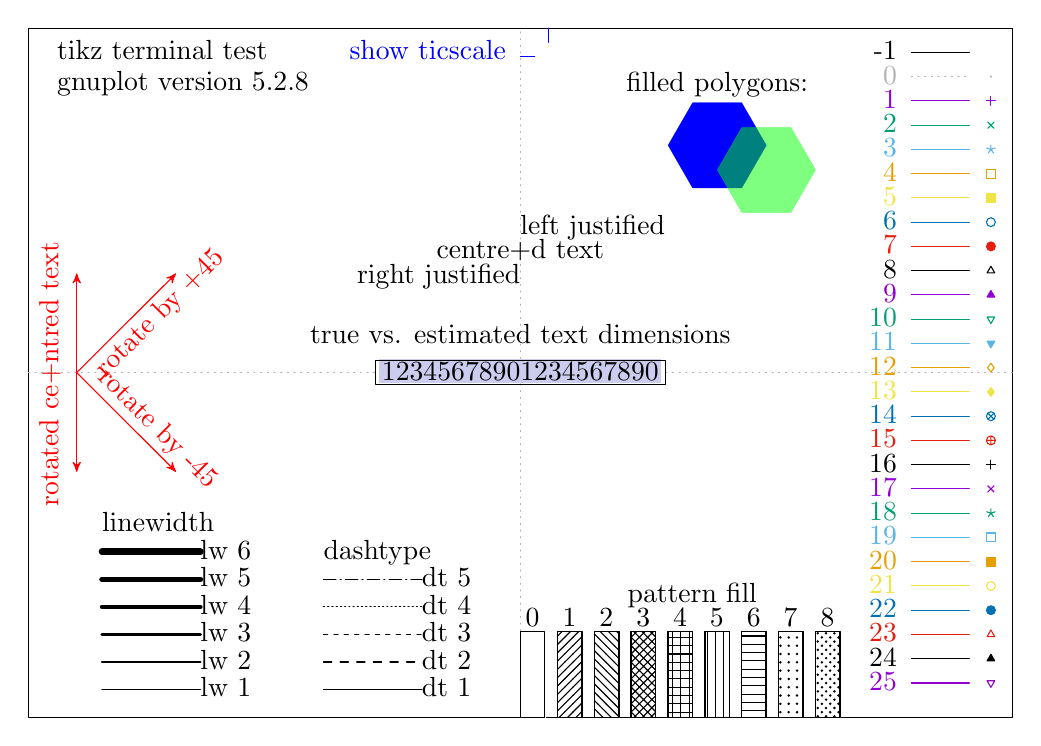
\begin{tikzpicture}[gnuplot]
%% generated with GNUPLOT 5.2p8 (Lua 5.3; terminal rev. Nov 2018, script rev. 108)
%% 2021年05月10日 22時42分14秒
\path (0.000,0.000) rectangle (12.500,8.750);
\gpcolor{color=gp lt color border}
\gpsetlinetype{gp lt border}
\gpsetdashtype{gp dt solid}
\gpsetlinewidth{1.00}
\draw[gp path] (0.000,0.000)--(12.499,0.000)--(12.499,8.749)--(0.000,8.749)--cycle;
\node[gp node left,inner sep=0pt](gp boxed node 62) at (0.368,8.442) {tikz  terminal test};
\node[gp node left,inner sep=0pt](gp boxed node 63) at (0.368,8.057) {gnuplot version 5.2.8  };
\gpcolor{color=gp lt color axes}
\gpsetlinetype{gp lt axes}
\gpsetdashtype{gp dt axes}
\draw[gp path] (6.250,0.000)--(6.250,8.749);
\draw[gp path] (0.000,4.375)--(12.499,4.375);
\gpcolor{color=gp lt color border}
\node[gp node center,inner sep=0pt](gp boxed node 1) at (6.250,4.375) {12345678901234567890};
\gpcolor{rgb color={0.800,0.800,0.933}}
\gpsetlinetype{gp lt border}
\gpsetdashtype{gp dt solid}
\node[fill={}, inner xsep=1.00, inner ysep=1.00,fit=(gp boxed node 1)]{};
\gpcolor{color=gp lt color border}
\node[gp node center,inner sep=0pt](gp boxed node 2) at (6.250,4.375) {12345678901234567890};
\node[gp node center,inner sep=0pt](gp boxed node 3) at (6.250,4.837) {true vs. estimated text dimensions};
\draw[gp path] (4.410,4.529)--(8.090,4.529)--(8.090,4.221)--(4.410,4.221)--cycle;
\node[gp node left,inner sep=0pt](gp boxed node 4) at (6.250,6.223) {left justified};
\node[gp node center,inner sep=0pt](gp boxed node 5) at (6.250,5.915) {centre+d text};
\node[gp node right,inner sep=0pt](gp boxed node 6) at (6.250,5.607) {right justified};
\gpcolor{color=gp lt color 2}
\gpsetlinetype{gp lt plot 2}
\draw[gp path] (6.610,8.749)--(6.610,8.570);
\draw[gp path] (6.250,8.390)--(6.430,8.390);
\node[gp node right,inner sep=0pt](gp boxed node 7) at (6.066,8.442) {show ticscale};
\gpcolor{color=gp lt color border}
\node[gp node right,inner sep=0pt](gp boxed node 8) at (11.032,8.442) {-1};
\gpsetlinetype{gp lt border}
\draw[gp path] (11.216,8.442)--(11.952,8.442);
\gpcolor{color=gp lt color axes}
\node[gp node right,inner sep=0pt](gp boxed node 9) at (11.032,8.134) {0};
\gpsetlinetype{gp lt axes}
\gpsetdashtype{gp dt axes}
\draw[gp path] (11.216,8.134)--(11.952,8.134);
\gpsetpointsize{4.00}
\gppoint{gp mark 0}{(12.226,8.134)}
\gpcolor{rgb color={0.580,0.000,0.827}}
\node[gp node right,inner sep=0pt](gp boxed node 10) at (11.032,7.826) {1};
\gpsetlinetype{gp lt border}
\gpsetdashtype{gp dt solid}
\draw[gp path] (11.216,7.826)--(11.952,7.826);
\gppoint{gp mark 1}{(12.226,7.826)}
\gpcolor{rgb color={0.000,0.620,0.451}}
\node[gp node right,inner sep=0pt](gp boxed node 11) at (11.032,7.518) {2};
\draw[gp path] (11.216,7.518)--(11.952,7.518);
\gppoint{gp mark 2}{(12.226,7.518)}
\gpcolor{rgb color={0.337,0.706,0.914}}
\node[gp node right,inner sep=0pt](gp boxed node 12) at (11.032,7.210) {3};
\draw[gp path] (11.216,7.210)--(11.952,7.210);
\gppoint{gp mark 3}{(12.226,7.210)}
\gpcolor{rgb color={0.902,0.624,0.000}}
\node[gp node right,inner sep=0pt](gp boxed node 13) at (11.032,6.902) {4};
\draw[gp path] (11.216,6.902)--(11.952,6.902);
\gppoint{gp mark 4}{(12.226,6.902)}
\gpcolor{rgb color={0.941,0.894,0.259}}
\node[gp node right,inner sep=0pt](gp boxed node 14) at (11.032,6.594) {5};
\draw[gp path] (11.216,6.594)--(11.952,6.594);
\gppoint{gp mark 5}{(12.226,6.594)}
\gpcolor{rgb color={0.000,0.447,0.698}}
\node[gp node right,inner sep=0pt](gp boxed node 15) at (11.032,6.286) {6};
\draw[gp path] (11.216,6.286)--(11.952,6.286);
\gppoint{gp mark 6}{(12.226,6.286)}
\gpcolor{rgb color={0.898,0.118,0.063}}
\node[gp node right,inner sep=0pt](gp boxed node 16) at (11.032,5.978) {7};
\draw[gp path] (11.216,5.978)--(11.952,5.978);
\gppoint{gp mark 7}{(12.226,5.978)}
\gpcolor{rgb color={0.000,0.000,0.000}}
\node[gp node right,inner sep=0pt](gp boxed node 17) at (11.032,5.670) {8};
\draw[gp path] (11.216,5.670)--(11.952,5.670);
\gppoint{gp mark 8}{(12.226,5.670)}
\gpcolor{rgb color={0.580,0.000,0.827}}
\node[gp node right,inner sep=0pt](gp boxed node 18) at (11.032,5.362) {9};
\draw[gp path] (11.216,5.362)--(11.952,5.362);
\gppoint{gp mark 9}{(12.226,5.362)}
\gpcolor{rgb color={0.000,0.620,0.451}}
\node[gp node right,inner sep=0pt](gp boxed node 19) at (11.032,5.054) {10};
\draw[gp path] (11.216,5.054)--(11.952,5.054);
\gppoint{gp mark 10}{(12.226,5.054)}
\gpcolor{rgb color={0.337,0.706,0.914}}
\node[gp node right,inner sep=0pt](gp boxed node 20) at (11.032,4.746) {11};
\draw[gp path] (11.216,4.746)--(11.952,4.746);
\gppoint{gp mark 11}{(12.226,4.746)}
\gpcolor{rgb color={0.902,0.624,0.000}}
\node[gp node right,inner sep=0pt](gp boxed node 21) at (11.032,4.438) {12};
\draw[gp path] (11.216,4.438)--(11.952,4.438);
\gppoint{gp mark 12}{(12.226,4.438)}
\gpcolor{rgb color={0.941,0.894,0.259}}
\node[gp node right,inner sep=0pt](gp boxed node 22) at (11.032,4.130) {13};
\draw[gp path] (11.216,4.130)--(11.952,4.130);
\gppoint{gp mark 13}{(12.226,4.130)}
\gpcolor{rgb color={0.000,0.447,0.698}}
\node[gp node right,inner sep=0pt](gp boxed node 23) at (11.032,3.822) {14};
\draw[gp path] (11.216,3.822)--(11.952,3.822);
\gppoint{gp mark 14}{(12.226,3.822)}
\gpcolor{rgb color={0.898,0.118,0.063}}
\node[gp node right,inner sep=0pt](gp boxed node 24) at (11.032,3.514) {15};
\draw[gp path] (11.216,3.514)--(11.952,3.514);
\gppoint{gp mark 15}{(12.226,3.514)}
\gpcolor{rgb color={0.000,0.000,0.000}}
\node[gp node right,inner sep=0pt](gp boxed node 25) at (11.032,3.206) {16};
\draw[gp path] (11.216,3.206)--(11.952,3.206);
\gppoint{gp mark 1}{(12.226,3.206)}
\gpcolor{rgb color={0.580,0.000,0.827}}
\node[gp node right,inner sep=0pt](gp boxed node 26) at (11.032,2.898) {17};
\draw[gp path] (11.216,2.898)--(11.952,2.898);
\gppoint{gp mark 2}{(12.226,2.898)}
\gpcolor{rgb color={0.000,0.620,0.451}}
\node[gp node right,inner sep=0pt](gp boxed node 27) at (11.032,2.590) {18};
\draw[gp path] (11.216,2.590)--(11.952,2.590);
\gppoint{gp mark 3}{(12.226,2.590)}
\gpcolor{rgb color={0.337,0.706,0.914}}
\node[gp node right,inner sep=0pt](gp boxed node 28) at (11.032,2.282) {19};
\draw[gp path] (11.216,2.282)--(11.952,2.282);
\gppoint{gp mark 4}{(12.226,2.282)}
\gpcolor{rgb color={0.902,0.624,0.000}}
\node[gp node right,inner sep=0pt](gp boxed node 29) at (11.032,1.974) {20};
\draw[gp path] (11.216,1.974)--(11.952,1.974);
\gppoint{gp mark 5}{(12.226,1.974)}
\gpcolor{rgb color={0.941,0.894,0.259}}
\node[gp node right,inner sep=0pt](gp boxed node 30) at (11.032,1.666) {21};
\draw[gp path] (11.216,1.666)--(11.952,1.666);
\gppoint{gp mark 6}{(12.226,1.666)}
\gpcolor{rgb color={0.000,0.447,0.698}}
\node[gp node right,inner sep=0pt](gp boxed node 31) at (11.032,1.358) {22};
\draw[gp path] (11.216,1.358)--(11.952,1.358);
\gppoint{gp mark 7}{(12.226,1.358)}
\gpcolor{rgb color={0.898,0.118,0.063}}
\node[gp node right,inner sep=0pt](gp boxed node 32) at (11.032,1.050) {23};
\draw[gp path] (11.216,1.050)--(11.952,1.050);
\gppoint{gp mark 8}{(12.226,1.050)}
\gpcolor{rgb color={0.000,0.000,0.000}}
\node[gp node right,inner sep=0pt](gp boxed node 33) at (11.032,0.742) {24};
\draw[gp path] (11.216,0.742)--(11.952,0.742);
\gppoint{gp mark 9}{(12.226,0.742)}
\gpcolor{rgb color={0.580,0.000,0.827}}
\node[gp node right,inner sep=0pt](gp boxed node 34) at (11.032,0.434) {25};
\draw[gp path] (11.216,0.434)--(11.952,0.434);
\gppoint{gp mark 10}{(12.226,0.434)}
\gpcolor{color=gp lt color 0}
\gpsetlinetype{gp lt plot 0}
\draw[gp path,<->](0.616,3.115)--(0.616,5.635);
\draw[gp path,->](0.616,4.375)--(1.876,5.635);
\draw[gp path,->](0.616,4.375)--(1.876,3.115);
\node[gp node center,rotate=-270,inner sep=0pt](gp boxed node 35) at (0.308,4.375) {rotated ce+ntred text};
\node[gp node left,rotate=45,inner sep=0pt](gp boxed node 36) at (0.924,4.375) {  rotate by +45};
\node[gp node left,rotate=-45,inner sep=0pt](gp boxed node 37) at (0.924,4.375) {  rotate by -45};
\gpcolor{color=gp lt color border}
\gpsetlinetype{gp lt border}
\draw[gp path] (0.937,0.350)--(2.187,0.350);
\node[gp node left,inner sep=0pt](gp boxed node 38) at (2.187,0.350) {  lw 1};
\gpsetlinewidth{2.00}
\draw[gp path] (0.937,0.700)--(2.187,0.700);
\node[gp node left,inner sep=0pt](gp boxed node 39) at (2.187,0.700) {  lw 2};
\gpsetlinewidth{3.00}
\draw[gp path] (0.937,1.050)--(2.187,1.050);
\node[gp node left,inner sep=0pt](gp boxed node 40) at (2.187,1.050) {  lw 3};
\gpsetlinewidth{4.00}
\draw[gp path] (0.937,1.400)--(2.187,1.400);
\node[gp node left,inner sep=0pt](gp boxed node 41) at (2.187,1.400) {  lw 4};
\gpsetlinewidth{5.00}
\draw[gp path] (0.937,1.750)--(2.187,1.750);
\node[gp node left,inner sep=0pt](gp boxed node 42) at (2.187,1.750) {  lw 5};
\gpsetlinewidth{6.00}
\draw[gp path] (0.937,2.100)--(2.187,2.100);
\node[gp node left,inner sep=0pt](gp boxed node 43) at (2.187,2.100) {  lw 6};
\node[gp node left,inner sep=0pt](gp boxed node 44) at (0.937,2.450) {linewidth};
\gpsetdashtype{gp dt 1}
\gpsetlinewidth{1.00}
\draw[gp path] (3.750,0.350)--(5.000,0.350);
\node[gp node left,inner sep=0pt](gp boxed node 45) at (5.000,0.350) {  dt 1};
\gpsetdashtype{gp dt 2}
\draw[gp path] (3.750,0.700)--(5.000,0.700);
\node[gp node left,inner sep=0pt](gp boxed node 46) at (5.000,0.700) {  dt 2};
\gpsetdashtype{gp dt 3}
\draw[gp path] (3.750,1.050)--(5.000,1.050);
\node[gp node left,inner sep=0pt](gp boxed node 47) at (5.000,1.050) {  dt 3};
\gpsetdashtype{gp dt 4}
\draw[gp path] (3.750,1.400)--(5.000,1.400);
\node[gp node left,inner sep=0pt](gp boxed node 48) at (5.000,1.400) {  dt 4};
\gpsetdashtype{gp dt 5}
\draw[gp path] (3.750,1.750)--(5.000,1.750);
\node[gp node left,inner sep=0pt](gp boxed node 49) at (5.000,1.750) {  dt 5};
\node[gp node left,inner sep=0pt](gp boxed node 50) at (3.750,2.100) {dashtype};
\node[gp node center,inner sep=0pt](gp boxed node 51) at (8.434,1.555) {pattern fill};
\def\gpfillpath{(6.250,0.000)--(6.562,0.000)--(6.562,1.093)--(6.250,1.093)--cycle}
\gpfill{color=gpbgfillcolor} \gpfillpath;
\gpfill{color=gp lt color border,gp pattern 0,pattern color=.} \gpfillpath;
\gpsetdashtype{gp dt solid}
\draw[gp path] (6.250,0.000)--(6.250,1.093)--(6.562,1.093)--(6.562,0.000)--cycle;
\node[gp node center,inner sep=0pt](gp boxed node 52) at (6.406,1.247) { 0};
\def\gpfillpath{(6.718,0.000)--(7.030,0.000)--(7.030,1.093)--(6.718,1.093)--cycle}
\gpfill{color=gpbgfillcolor} \gpfillpath;
\gpfill{color=gp lt color border,gp pattern 1,pattern color=.} \gpfillpath;
\draw[gp path] (6.718,0.000)--(6.718,1.093)--(7.030,1.093)--(7.030,0.000)--cycle;
\node[gp node center,inner sep=0pt](gp boxed node 53) at (6.874,1.247) { 1};
\def\gpfillpath{(7.186,0.000)--(7.498,0.000)--(7.498,1.093)--(7.186,1.093)--cycle}
\gpfill{color=gpbgfillcolor} \gpfillpath;
\gpfill{color=gp lt color border,gp pattern 2,pattern color=.} \gpfillpath;
\draw[gp path] (7.186,0.000)--(7.186,1.093)--(7.498,1.093)--(7.498,0.000)--cycle;
\node[gp node center,inner sep=0pt](gp boxed node 54) at (7.342,1.247) { 2};
\def\gpfillpath{(7.654,0.000)--(7.966,0.000)--(7.966,1.093)--(7.654,1.093)--cycle}
\gpfill{color=gpbgfillcolor} \gpfillpath;
\gpfill{color=gp lt color border,gp pattern 3,pattern color=.} \gpfillpath;
\draw[gp path] (7.654,0.000)--(7.654,1.093)--(7.966,1.093)--(7.966,0.000)--cycle;
\node[gp node center,inner sep=0pt](gp boxed node 55) at (7.810,1.247) { 3};
\def\gpfillpath{(8.122,0.000)--(8.434,0.000)--(8.434,1.093)--(8.122,1.093)--cycle}
\gpfill{color=gpbgfillcolor} \gpfillpath;
\gpfill{color=gp lt color border,gp pattern 4,pattern color=.} \gpfillpath;
\draw[gp path] (8.122,0.000)--(8.122,1.093)--(8.434,1.093)--(8.434,0.000)--cycle;
\node[gp node center,inner sep=0pt](gp boxed node 56) at (8.278,1.247) { 4};
\def\gpfillpath{(8.590,0.000)--(8.902,0.000)--(8.902,1.093)--(8.590,1.093)--cycle}
\gpfill{color=gpbgfillcolor} \gpfillpath;
\gpfill{color=gp lt color border,gp pattern 5,pattern color=.} \gpfillpath;
\draw[gp path] (8.590,0.000)--(8.590,1.093)--(8.902,1.093)--(8.902,0.000)--cycle;
\node[gp node center,inner sep=0pt](gp boxed node 57) at (8.746,1.247) { 5};
\def\gpfillpath{(9.058,0.000)--(9.370,0.000)--(9.370,1.093)--(9.058,1.093)--cycle}
\gpfill{color=gpbgfillcolor} \gpfillpath;
\gpfill{color=gp lt color border,gp pattern 6,pattern color=.} \gpfillpath;
\draw[gp path] (9.058,0.000)--(9.058,1.093)--(9.370,1.093)--(9.370,0.000)--cycle;
\node[gp node center,inner sep=0pt](gp boxed node 58) at (9.214,1.247) { 6};
\def\gpfillpath{(9.526,0.000)--(9.838,0.000)--(9.838,1.093)--(9.526,1.093)--cycle}
\gpfill{color=gpbgfillcolor} \gpfillpath;
\gpfill{color=gp lt color border,gp pattern 7,pattern color=.} \gpfillpath;
\draw[gp path] (9.526,0.000)--(9.526,1.093)--(9.838,1.093)--(9.838,0.000)--cycle;
\node[gp node center,inner sep=0pt](gp boxed node 59) at (9.682,1.247) { 7};
\def\gpfillpath{(9.994,0.000)--(10.306,0.000)--(10.306,1.093)--(9.994,1.093)--cycle}
\gpfill{color=gpbgfillcolor} \gpfillpath;
\gpfill{color=gp lt color border,gp pattern 8,pattern color=.} \gpfillpath;
\draw[gp path] (9.994,0.000)--(9.994,1.093)--(10.306,1.093)--(10.306,0.000)--cycle;
\node[gp node center,inner sep=0pt](gp boxed node 60) at (10.150,1.247) { 8};
\gpfill{color=gp lt color 2} (9.375,7.262)--(9.062,7.803)--(8.437,7.803)--(8.125,7.262)%
    --(8.437,6.720)--(9.062,6.720)--cycle;
\gpfill{color=gp lt color 1,opacity=0.50} (10.000,6.950)--(9.687,7.491)--(9.062,7.491)--(8.750,6.950)%
    --(9.062,6.408)--(9.687,6.408)--cycle;
\node[gp node center,inner sep=0pt](gp boxed node 61) at (8.750,8.041) {filled polygons:};
%% coordinates of the plot area
\gpdefrectangularnode{gp plot 1}{\pgfpoint{1.805cm}{1.723cm}}{\pgfpoint{18.655cm}{18.573cm}}
\end{tikzpicture}
%% gnuplot variables

  \end{center}
\end{figure}

\bibliography{ref.bib}
\end{document}